\chapter{Core Lines in 3D Second-Order Tensor Fields} % (fold)
\label{cha:tensor_core_lines}
%
\tikzset{external/export=false}
\begin{tikzpicture}[remember picture, overlay]
    \node[paperheader]
        at ([yshift=1.2cm]mychapanchor-\arabic{chapter} -| current page text area.west)
        (banner_fst) {%
            \parbox[b]{0.5\textwidth}{%
            This chapter is based on the publication:\\
            \fullcite{Oster2018}}
    };
\end{tikzpicture}
\tikzset{external/export=true}
%
\vspace{-\baselineskip}\lettrine[lhang=0.03, loversize=-0.015]{V}{ortex core
lines} describe the centers of swirling behavior in vector fields.
%
They are a useful tool in vector field visualization because they provide an
explicit geometrical representation of an important flow feature.
%
Different definitions and strategies for extracting vortex core lines have been
presented in \cref{sub:vortex_extraction}.
%
One of the simplest and most popular methods is the one proposed by Sujudi and
Haimes~\cite{Sujudi1995}, which can be computed using the \ac{PV}
operator~\cite{Peikert1999}.
%

%
Tensor field lines, \ie{}, lines that are everywhere tangential to an eigenvector
of a tensor field (see \cref{sub:tensor_line_surface_based}), can also exhibit
``swirling'' behavior similar to vortices in vector fields.
%
For example, stress tensor fields show stress trajectories winding around a
common core in regions of twist.
%
Various visualization methods for tensor fields exist, but to date no approach
has been proposed to extract core lines of such vortex-like structures.
%

%
As we have already explained in \cref{cha:parallel_eigenvectors}, simply using
the Sujudi/Haimes criterion and applying the \ac{PV} operator to the
``eigenvector fields'' of the data cannot give consistent results.
%
We therefore introduce \emph{tensor core lines} as an equivalent to vortex
core lines in vector fields.
%
Their definition is a direct extension of the Sujudi/Haimes criterion to tensor
fields and their extraction is based on the \ac{PEV} operator.
%
\begin{figure}[t]
    \centering
    \setlength\figurewidth\textwidth
    \begin{tikzpicture}[
    every node/.style={inner sep=0, outer sep=0},
]
    \node (img) at (0,0) {
        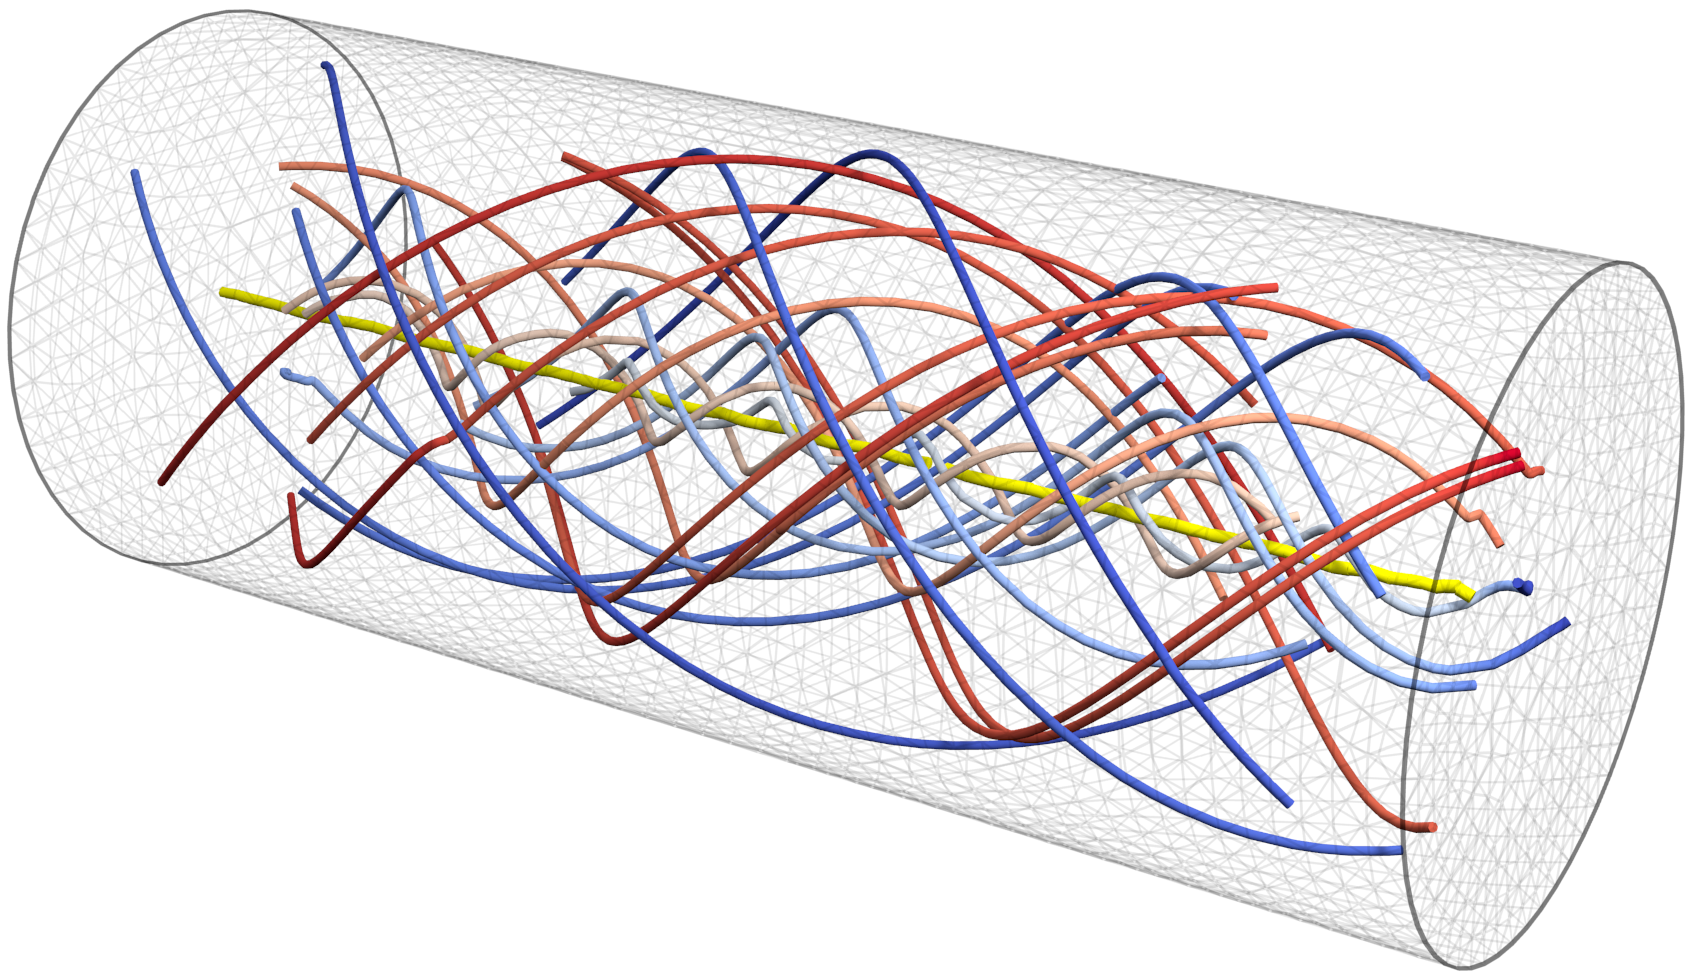
\includegraphics[width=\figurewidth]{figures/torque_tube_lines.png}
    };
    \begin{scope}[
        shift=(img.south west), % origin is lower left corner
        x={($(img.south east)-(img.south west)$)}, % x axis is lower side
        y={($(img.north west)-(img.south west)$)}] % y axis is left side
        % uncomment the following three lines to show a helper grid that helps
        % with finding coordinates
        % \draw[help lines, opacity=0.5, xstep=.01,ystep=.01] (0,0) grid (1,1);
        % \draw[thin, xstep=.1,ystep=.1] (0,0) grid (1,1);
        % \foreach \x in {0,...,9} { \node [anchor=north] at (\x/10,0) {0.\x}; }
        % \foreach \y in {0,...,9} { \node [anchor=east] at (0,\y/10) {0.\y}; }
        % draw stuff on image
        % (0, 0) is lower left corner, (1, 1) is upper right
        \node at (0.916,0.37) {
            \begin{tikzpicture}
                \draw[-latex, ultra thick, black, rotate=76] (0,0)
                arc[x radius = 2.6cm, y radius = 0.8cm, start angle= 60, end angle= -255];
            \end{tikzpicture}
        };

        \node at (0.123,0.705) {
            \begin{tikzpicture}
                \draw[-latex, ultra thick, black, rotate=76] (0,0)
                arc[x radius = 2.02cm, y radius = 1.385cm, start angle= -255, end angle= 60];
            \end{tikzpicture}
        };
    \end{scope}
\end{tikzpicture}
    % \vspace*{-9mm}
    \caption{Tensor field lines in a stress tensor field induced by
             applying a torque to a cylindrical shaft. Field lines of both major
             (blue) and minor (red) eigenvectors show a swirling behavior around
             a common core line (yellow).}
    \label{fig:tube_lines}
\end{figure}
%
In particular, we make the following contributions:
%
\begin{itemize}
    \item  We give a rigorous definition of tensor core lines and show that
    indeed the definition gives structurally stable line structures.
    %
    \item We provide a numerical algorithm for the extraction of tensor core
    lines from piecewise linear tensor fields.
    %
    \item We introduce a filter criterion based on numerical stability to
    separate significant and insignificant tensor core lines.
    %
    \item We show tensor core lines in mechanical stress tensor fields,
    interpret them and compare them with degenerate lines where two eigenvalues
    are equal.
\end{itemize}
%
We introduce tensor core lines in \cref{sec:tcl_theory} and study their
properties.
%
We then present our algorithm for extracting tensor core lines in
\cref{sec:extracting_tensor_lines}.
%
We show our results on several stress tensor fields in \cref{sec:tcl_results}
and study the performance, robustness and relation to degenerate lines.
%
As it turns out, our algorithm is sufficiently generic to be applied to the
extraction of \ac{PEV} lines and degenerate lines as well.
%
We show how this can be done in \cref{sec:computing_pev_and_degenerate_lines}
and close with a discussion in \cref{sec:tcl_discussion}.
%
% section introduction (end)
%
% 
%
\section{Related Work} % (fold)
\label{sec:tcl_related_work}
%
The basis of this work is the extractor for centers of swirling flow in vector
fields first described by Sujudi and Haimes~\cite{Sujudi1995}.
%
In their original paper, they examine the Jacobian $\nabla \vv$ of a vector
field $\vv$.
%
They search for vortex core lines only in areas where $\nabla \vv$ has two
complex eigenvalues, \ie, where the flow shows locally swirling behavior.
%
The location of a vortex core line is then defined as the set of points where
the velocity is parallel to the single real eigenvector.
%
These are the locations where the swirling in the orthogonal plane vanishes
and only a motion along the eigenvector direction remains.
%
Note that vortex core lines defined in this manner are generally not streamlines
of the vector field.
%
When applying this method to a piecewise linear vector field, the result is a
set of straight line segments.
%
Since the derivative $\nabla \vv$ is constant within each cell, these segments
do not generally form closed lines.
%
Single line segments may appear due to noise, but if multiple line segments form
a visually coherent line, it is a strong indicator for vortical behavior in the
flow.
%
The advantage of this vortex core line extractor is its inherent locality, which
makes it well-suited for parallelization and avoids expensive line integration.
%
%
\subsection*{Parallel Vectors} % (fold)
\label{sub:tcl_parallel_vectors}
%
Peikert and Roth~\cite{Peikert1999} showed that the vortex core lines described
by Sujudi and Haimes are locations where the acceleration $\nabla \vv \cdot \vv$
is parallel to the vector field, and identified this as one application of a
concept they called the \emph{parallel vectors operator}.
%
This concept had been applied in a lot of other contexts before, such as ridge
detection in scalar fields~\cite{Haralick1983} and extraction of
attachment/separation lines in flows~\cite{Kenwright1999}.
%

%
An overview of a number of algorithms for computing parallel vectors can be
found in Martin Roth's PhD thesis~\cite{Roth2000}.
%
A common approach is to first determine intersection points of the \ac{PV} lines
with the cell faces of a data set.
%
The resulting points are then connected to lines.
%
If there are exactly two intersections with the faces of a cell, they can be
trivially connected with a line.
%
In case of a higher number of intersections, different heuristics have been
employed, the simplest one being to subdivide the cell until there are again
only two intersections.
%

%
Another class of algorithms employs some form of line tracing to follow a
parallel vector line starting from a seed point that has been found by one of
the aforementioned face intersection methods.
%
Banks and Singer~\cite{Banks1995} and Miura and Kida~\cite{Miura1997} employed a
predictor-corrector scheme, following the lines in small steps and minimizing
the angle between the vector fields in an orthogonal plane after each step.
%
Sukharev et al.~\cite{Sukharev2006} presented a mix between both approaches by
first finding intersection points on a (potentially coarser) grid, and then
following the analytical tangent of the \ac{PV} line to connect them.
%
A similar approach is taken by Theisel et al.~\cite{Theisel2003a}, where the
\ac{PV} line is reformulated as a stream line in a {\em feature flow field} that is
derived from the original vector fields.
%
Given a starting point on the \ac{PV} line, it can be traced like a stream line with
any standard ODE solver.
%
The \emph{PVsolve} framework introduced by van Gelder and Pang~\cite{Gelder2009}
is a generalized approach for finding \ac{PV} lines in vector fields of different
dimensionality.
%
Their approach views the tracing of \ac{PV} lines as a root-finding problem and
presents an algorithm that does not suffer from accumulating errors.
%
Weinkauf et al.~\cite{Weinkauf2011} presented stable feature flow fields as an
extension to feature flow fields that similarly eliminates accumulating errors.
%

%
Most \ac{PV} algorithms assume they operate on piecewise linear or piecewise
bi-/trilinear data in two- or three-dimensional space.
%
However, there have been a number of publications dealing with higher-order data
or using higher-order methods in some form.
%
Roth and Peikert~\cite{Roth1998} introduced a method for finding strongly curved
vortex core lines by using higher-order derivatives of the flow field.
%
Bauer and Peikert~\cite{Bauer2002} used a scale-space technique to filter out
small-scale structures and irrelevant large-scale ones when computing vortex
cores.
%
Pagot et al.~\cite{Pagot2011} presented an algorithm for extracting \ac{PV} lines
from data represented by higher-order basis functions.
%
Due to its generality, the already mentioned \emph{PVsolve}
framework~\cite{Gelder2009} allows for extracting parallel vector surfaces in
time-dependent vector fields.
%
Similarly, Theisel at al.~\cite{Theisel2005} extracted \ac{PV} surfaces in unsteady
flows and applied it to vortex core line tracking.
%
All these methods work on vector fields, while our approach deals with
second-order tensor fields.
%
% subsection parallel_eigenvectors (end)

\subsection*{Tensor Field Visualization} % (fold)
\label{sub:tcl_tensor_field_visualization}
%
Tensor fields (of second order) occur in a variety of different scientific
contexts.
%
Some examples are stress and strain tensors in mechanical engineering
applications, and diffusion tensors occuring in \ac{DTI}, a special \ac{MRI}
modality used to visualize fiber tracts, \eg, in the human brain.
%
Tensor field visualization methods can be roughly classified into three
different categories:
%
glyph-based, line-/surface-based and topology-based.
%

%
Glyph-based methods for tensor field visualization place small geometric objects
in space to represent certain characteristics of the local tensor.
%
Diffusion tensors, which are symmetric and positive definite, have been
visualized by Kindlmann~\cite{Kindlmann2004} using superquadric glyphs
aligned with the eigenvector directions.
%
By explicitly encoding eigenvalue signs in geometry, Schultz and
Kindlmann~\cite{Schultz2010a} extended this to indefinite tensors.
%
Gerrits \etal~\cite{Gerrits2017} additionally incorporated complex eigenvalue
information into the glyph design to visualize general second-order tensors
in \ac{2D} and \ac{3D}.
%
A specialized glyph for stress and strain tensors was introduced by Hashash
\etal~\cite{Hashash2003}.
%
Kindlmann and Westin~\cite{Kindlmann2006} addressed the problem of clutter by
optimizing glyph placement to increase information density while minimizing
occlusion.
%
Glyphs for comparative visualization of two different diffusion tensors were
used on medical data by Zhang \etal~\cite{Zhang2016}.
%

%
A simple extension of streamlines for visualizing symmetric tensor fields in \ac{3D}
are hyperstreamlines, first introduced by Delmarcelle and
Hesselink~\cite{Delmarcelle1993}.
%
These hyperstreamlines follow one of the eigenvectors of the tensor field, while
their cross-section is a cross shape or ellipse aligned with the other two
eigenvectors and scaled by the corresponding eigenvalues.
%
The problem of undefined integration direction in near-isotropic areas was
adressed by Weinstein \etal with a new concept called
tensorlines~\cite{Weinstein1999}.
%
These lines behave like hyperstreamlines, but try to preserve direction in areas
of equal eigenvalues by incorporating local context information.
%
As an extension to this concept, Jeremi{\'c} \etal introduced
hyperstreamsurfaces~\cite{Jeremic2002}, which are formed analogous to
hyperstreamlines by using a line instead of a point as the seed structure.
%

%
The topology of symmetric \ac{2D} and \ac{3D} tensor fields was studied by
Delmarcelle~\cite{Delmarcelle1994} and Hesselink~\cite{Hesselink1997}.
%
They characterized the topology of a tensor field by degenerate structures
where two or more eigenvalues are equal.
%
Zheng and Pang~\cite{Zheng2004} build on top of this work and provide
numerical algorithms for extracting the topological skeleton in practice.
%
Similar to the approach we take for extracting tensor core lines, their initial
algorithm is based on finding the roots of a number of discriminant functions on
the cell faces of a dataset using a bisection algorithm, and then connecting
them to lines.
%
Zheng \etal later introduced alternative approaches that are based on solving
a system of equations on each face, and on tracing the degenerate lines using
their analytical tangent~\cite{Zheng2005}.
%
As Schulz \etal~\cite{Schultz2007} showed, these features are very sensitive to
noise.
%
A more stable approach suitable to noisy data such as obtained from DTI scans
was therefore proposed by Tricoche \etal~\cite{Tricoche2008}.
%
The notion of tensor topology was recently extended to surfaces of neutral and
traceless tensors by Palacios \etal~\cite{Palacios2016}, who also propose an
improved algorithm for extracting degenerate lines.
%
Assymetric tensors were studied in 2D by Zheng and Pang~\cite{Zheng2005a} and
in the context of flow visualization by Zhang \etal~\cite{Zhang2009}.
%
% - Gordon on derivatives of eigenvectors
% section related_work (end)
%
% 
%
\section{Notation} % (fold)
\label{sec:tcl_notation}
% 
Throughout the paper, we use the following notation:
%

%
\noindent
\begin{tabular}{ll}
$\mT$ & Matrix in $\RRSet^{3 \times 3}$\\
$\vv$ & Column vector in $\RRSet^3$ \\
$v_i$ & Components of a vector \\
$\begin{pmatrix} \va & \vb & \vc \end{pmatrix}$ & Block matrix of multiple matrices/vectors \\
$\mT_{x_1}, \vv_{x_2},...$ & Partial derivatives of a Matrix/vector in $x_1, x_2, \dots$ \\
$\nabla$ & Nabla operator $\T{(\frac{\partial}{\partial x_1}, \frac{\partial}{\partial x_2}, \frac{\partial}{\partial x_3}, \dots)}$\\
$\nabla_\vr\, \mF$ & Directional derivative of $\mF$ along a vector $\vr$\\
$\vv \parallel \vu$ & The PV operator applied to $\vv$ and $\vu$
\end{tabular}
% 
% section notation (end)
%
\section{Tensor Core Lines} % (fold)
\label{sec:tcl_theory}
%
The Sujudi/Haimes criterion defines a vortex core line as a structure on which
streamlines have a locally vanishing curvature.
%
The intuition is that in a region where streamlines show a swirling behavior,
there must be a center of rotation where the swirl vanishes.
%
This is fulfilled where the acceleration vector $\mJ\,\vv$ is parallel to the
velocity $\vv$, \ie{}, the flow is accelerated on a straight line.
%
Using this formulation, the criterion can be expressed in terms of the \ac{PV}
operator.
%
To only extract vortex core lines, the Sujudi/Haimes criterion requires an
additional filter criterion.
%
Vortices only occur in regions with swirling flow behavior, which is indicated
by the presence of complex eigenvalues of the Jacobian.
%
Zero-curvature lines also occur in regions where the Jacobian has three real
eigenvalues.
%
These hyperbolic trajectories are the centers of simultaneous converging and
diverging behavior of the vector field and can be used to extract Lagrangian
coherent structures~\cite{Machado2013,Machado2016}
%

%
We apply the idea of Sujudi/Haimes to tensor fields by looking for locations
where the curvature of tensor field lines locally vanishes.
%
We define tensor core lines as the locations where tensor field lines have a
locally vanishing curvature.
%
Note that like vortex core lines, tensor core lines are not generally field
lines of the tensor field.
%
In this section, we provide a formal definition of tensor core lines and
examine their mathematical properties.
%

\subsection{Definition} % (fold)
\label{sub:tcl_definition}
%
Let $\mT(\vx)$ be a \ac{3D} second-order tensor
field that may or may not be symmetric.
%
We want to find locations where the direction of a real eigenvector of $\mT$
does not change when moving along the eigenvector direction, \ie{}, where the
curvature of a tensor field line vanishes.
%
A vector $\vr \neq \vNull$ is a real eigenvector of $\mT$ if $\mT\,\vr = \lambda
\vr$ for eigenvalue $\lambda \in \RRSet$.
%
To observe the change of eigenvector direction when moving along $\vr$,
we need to consider the derivative of $\mT$ in this direction.
%
The directional derivative of $\mT$ along $\vr$, which we write as $\nabla_\vr
\mT$, is the linear combination of three component-wise derivatives
%
\begin{equation*}
    \nabla_{\vr}\mT(\vx) = \nabla \mT(\vx)\,\vr
        = \frac{\partial \mT(\vx)}{\partial x_1} r_1
        + \frac{\partial \mT(\vx)}{\partial x_2} r_2
        + \frac{\partial \mT(\vx)}{\partial x_3} r_3 \,\text{,}
\end{equation*}
%
for $\vx = \T{(x_1, x_2, x_3)}$ and $\vr = \T{(r_1, r_2, r_3)}$.
%

%
Given $\nabla_{\vr}\mT$ we can approximate the behavior of $\mT$ along
$\vr$ as
%
\begin{equation}
\label{eq:lin_approx}
    \mT(\vx + h\vr) = \mT(\vx) + h \nabla_{\vr}\mT(\vx) \,\text{,}
        \quad \text{with} \quad h \in \RRSet \,\text{.}
\end{equation}
%
For our zero-curvature requirement to be fulfilled, the eigenvector direction
must not change when moving along $\vr$, \ie{},
%
\begin{equation}
\label{eq:lin_cond}
    \mT(\vx + h\vr)\,\vr
        = \mT(\vx)\,\vr + h \nabla_{\vr}\mT(\vx)\,\vr
        = \mu \vr\, \text{,} \quad \text{with} \quad \mu \in \RRSet \,\text{.}
\end{equation}
%
This means that $\vr$ is still an eigenvector of $\mT$ (with eigenvalue $\mu$)
at the slightly offset position $\vx + h\vr$.
%
If we substitute $\mT(\vx)\,\vr = \lambda \vr$, we get
%
\begin{align*}
    \lambda \vr + h \nabla_{\vr}\mT(\vx)\,\vr &= \mu\, \vr \\
    \nabla_{\vr}\mT(\vx)\,\vr &= \frac{\mu-\lambda}{h}\, \vr\, \text{,}
\end{align*}
%
\ie{}, $\vr$ is also an eigenvector of $\nabla_{\vr} \mT(\vx)$.
%
With this, a tensor core line is an isolated line of positions $\vx$ where
%
\begin{equation*}
    \lambda \mT(\vx) \, \vr = \mu \nabla_{\vr}\mT(\vx)\,\vr = \vr \text{,}
\end{equation*}
%
for $\vr \neq \vNull$ and $\lambda,\, \mu \in \RRSet$.
%
In terms of the \ac{PV} operator, tensor core lines can then be expressed as
%
\begin{equation}
\label{eq:tensor_line}
    \operatorname{TCL}(\mT) =
        \{\vx\;|\: \exists \;\vr \in \RRSet,\,
        \vr \parallel \mT(\vx)\,\vr \parallel \nabla_{\vr}\mT(\vx)\,\vr
        \land \vr \neq \vNull\} \,\text{.}
\end{equation}
%
In words: a tensor core line is located where an eigenvector $\vr$ of $\mT$ is
parallel to an eigenvector of the directional derivative of $\mT$ along $\vr$.
%
Note the similarity of this criterion to Sujudi/Haimes, which states that a
vortex core lines is located where a vector $\vv$ of the vector field is
parallel to the directional derivative of the field along $\vv$, which is
defined by the acceleration $\mJ(\vv)\,\vv$.
%
In fact, the criterion is almost a straightforward application of the \ac{PEV}
operator we presented in \cref{cha:parallel_eigenvectors}.
%
However, the second tensor field $\nabla_{\vr}\mT$ is dependent on the unknown
$\vr$, which requires a slightly different solution strategy.
%

\begin{figure}
    \begin{captionbeside}
        {Example of seven distinct core lines in a random linear tensor field.
        \label{fig:7lines}}
        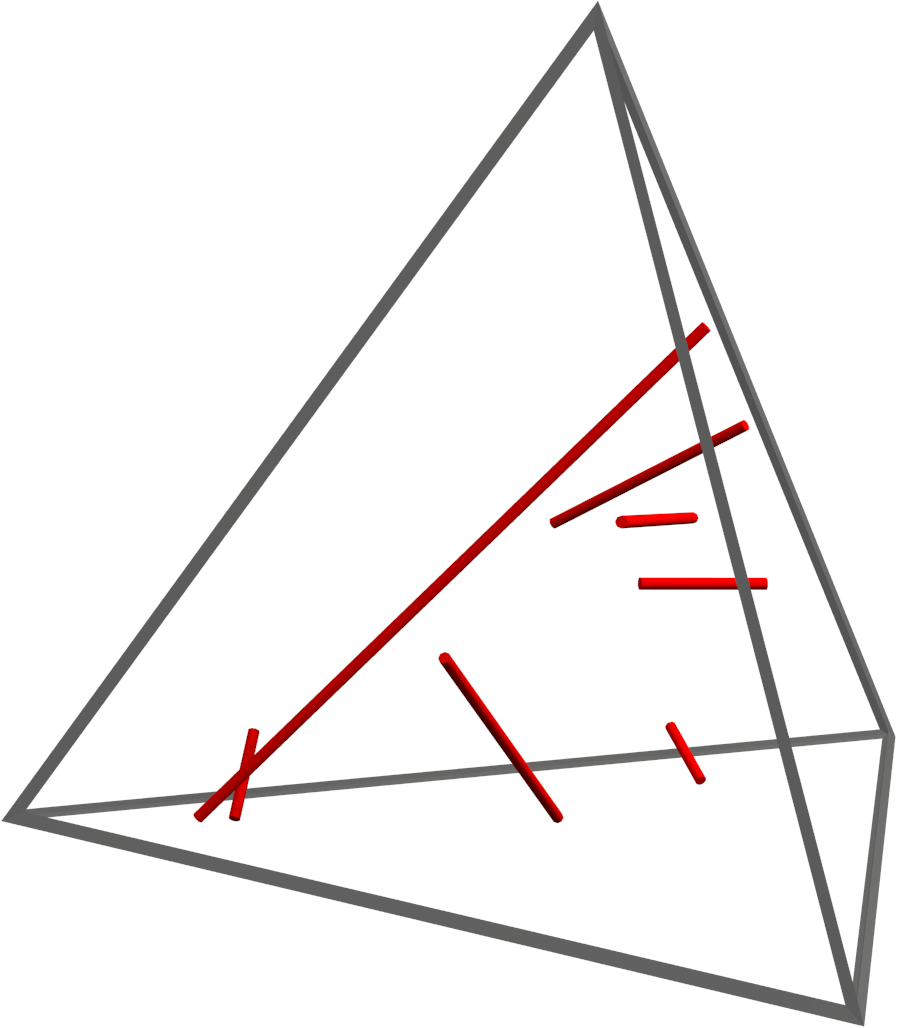
\includegraphics[width=0.5\columnwidth]{figures/7lines}
    \end{captionbeside}
\end{figure}
%
% subsection definition (end)

\subsection{Mathematical Properties} % (fold)
\label{sub:mathematical_properties}
%
We now examine the mathematical properties of tensor core lines.
%
We show that they are indeed structurally stable lines, and that in linear
tensor fields, these lines are always straight.
%

%
\begin{theorem}\label{thm:tcl_stable_lines}
In a $C^1$-continuous tensor field, tensor core lines are structurally stable
line structures that are either closed or end at the domain boundary.
\end{theorem}
%
To show \cref{thm:tcl_stable_lines}, we consider a local representation of a
real eigenvector field in the neighborhood of a point as a normalized vector
field.
%
Then the fact that the \ac{PV} operator gives such line
structures~\cite{Peikert1999} shows the theorem.
%
Note that although such a representation of an eigenvector field as a normalized
vector field is locally possible, it does not apply globally in a consistent
way, and therefore does not provide a strategy to extract tensor core lines.
%
We also mention that in real datasets, tensor cores may build surfaces or even
volumetric structures.
%
This is due to shape symmetries often observed in artificial data produced by
humans.
%
Even though these structures are unstable (adding noise destroys the surfaces to
many lines), our extraction algorithm has to deal with them.
%

%
\begin{theorem}
In linear tensor fields, tensor core lines are straight lines.
\end{theorem}
%
This follows from the fact that for linear tensor fields, the linear
approximation in \eqref{eq:lin_approx} describes the whole data set
exactly: if \eqref{eq:lin_cond} holds for a small $h$, it holds for all
$h$ (i.e., on a whole straight line) as well.
%
\Cref{fig:7lines} shows an example of a random linear tensor field containing
seven isolated tensor core lines.
%
% subsection mathematical_properties (end)
%

%
\section{Extracting Tensor Core Lines from Piecewise Linear Data} % (fold)
\label{sec:extracting_tensor_lines}
%
We assume tetrahedral partition of the three-dimensional domain.
%%
Each tetrahedron supports a linear piece if the given tensor field has a
constant tensor for each vertex.
%%
The gradient field $\nabla\mT$ consists of constant pieces per
tetrahedron.
%%

%
In general, tensor core structures are line features (see \cref{sec:tcl_theory}).
%%
We extract them by first bounding the search space to individual
tetrahedral cells and then to the cell boundary.
%%
The two-dimensional search on triangles reduces the extraction
generally to finding point features: the intersection of core lines
with the cell boundary.
%%
We will apply a root finding algorithm for feature extraction.
%%

%
This discretization of the field and also the restriction to a local
two-dimensional search space is applied similarly by other methods,
\eg, the Sujudi and Haimes extractor~\cite{Sujudi1995} or the extractor for
degenerate lines in tensor fields by Zheng and Pang~\cite{Zheng2004}.
%%
\subsection{General Algorithm}
%%
A tensor core line consists of all locations $\vx$ where
$\mT(\vx)\, \vr \parallel \vr$ and $\nabla_{\vr}\mT(\vx)\, \vr \parallel \vr$,
see \eqref{eq:tensor_line}.
%%
This can be expressed as solutions to
%%
\begin{equation}\label{eq:system}
\begin{aligned}
  (\mT(\vx)\,\vr) \times \vr &= \vNull\\
  (\nabla_{\vr} \mT(\vx)\, \vr) \times \vr &= \vNull~.
\end{aligned}
\end{equation}
%%
This system consists of six polynomial equations in the unknown
variables $\vx$ and $\vr\neq{}\vNull$.
%%

The polynomials are of maximum degree 1 in $\vx$ and 3 in $\vr$.
%%
Note that for a linear tensor field, $\nabla_{\vr}\mT(\vx)=\nabla_{\vr}\mT$ is
constant and thus independent of $\vx$.
%%
We parameterize directions $\vr$ such that they can be defined \wrt triangles.
%%
With the restriction of the local search space to triangles that bound
tetrahedra, the solution of the polynomial system is equivalent to
finding isolated (real) roots, \ie, points where all six polynomials
simultaneously become zero.
%%

%
We construct a bisection algorithm that uses the Bernstein-B\'ezier form
(\cref{sec:bb}) of the polynomials to exclude the presence of roots within
subtriangles.
%%
Within the search space (\cref{sec:searchspace}) a recursive
subdivision (\cref{sec:subdiv}) approximates the locations of roots in
$\vx$-$\vr$-space with an arbitrary user-defined precision.
%%
The local feature extraction is followed by a stage that clusters solutions and
then connects feature points to lines within cells (\cref{sec:cluster})
%
Finally, we use a filtering criterion for removing unstable solutions
(\cref{sec:filt}).
%
\subsection{Polynomial System in Bernstein-B\'ezier Form}
\label{sec:bb}
%%
We consider bivariate polynomials $p\,:\,\RRSet^2\rightarrow\RRSet$ of
degree $n$, which are evaluated in a triangular domain
$\Delta\subset\RRSet^2$.
%%
Let indices $i,j,k\geq{}0$.
%%
We write $p(\vu)$ in Bernstein-B\'ezier form as
%%
\begin{equation}\label{eq:bb}
\begin{aligned}
  p(\vu)~=\sum _{i+j+k=n} B^n_{ijk}(\vu)\,b_{ijk}~,\quad%
  B^n_{ijk}(\vu)~=~\frac{n!}{i!j!k!}\,a_1^i\,a_2^j\,a_3^k
\end{aligned}
\end{equation}
%%
with the bivariate Bernstein polynomials $B^n_{ijk}$ as basis and
coefficients (or B\'ezier control points) $b_{ijk}$.
%%
The basis is defined w.r.t. the barycentric coordinates
$a_\ell:=a_\ell(\vu)$, the linear polynomials that satisfy
%%
% \begin{equation}\label{eq:bc}
% \begin{aligned}
%   \sum _{\ell=1}^3 a_{\ell}(\vu)\,\vu_{\ell} = \vu\quad\text{and}\quad
%   \sum _{\ell=1}^3 a_{\ell}(\vu) = 1~.
% \end{aligned}
% \end{equation}
%%
\begin{equation}\label{eq:bc}
\begin{aligned}
a_1\vu_1+a_2\vu_2+a_3\vu_3 = \vu\quad\text{and}\quad
a_1+a_2+a_3 = 1
\end{aligned}
\end{equation}
\wrt triangle $\Delta$ spanned by vertices $\vu_1,\vu_2,\vu_3$
\cite{Hoschek1993}.
%%

%
The Bernstein-B\'ezier representation has a number of remarkable
properties.
%%
Important to our setting is the \emph{convex hull property}\/:
%%
For any $\vu\in\Delta$ -- or equivalently all barycentric coordinates
are nonnegative -- the value $p(\vu)$ is bounded by the convex hull
of the control points $b_{ijk}$.
%%
For scalar coefficients $b_{ijk}\in\RRSet$ this means that if either
all $b_{ijk}>0$ or all $b_{ijk}<0$ for $i+j+k=n$ then $p$
\emph{cannot} have a zero crossing (or real root) on $\Delta$.
%%
We use this criterion for an iterative subdivision of a triangle
$\Delta$ into smaller and smaller triangles that either may contain or
cannot contain a root.
%%
\subsection{Parameterization of the Search Space}
\label{sec:searchspace}
%%
The equations in the system~\eqref{eq:system} are polynomials in $\vx$
and $\vr$.
%%
This means the search space consists of two independent domains:
position and direction.
%%

%
As pointed out before, positions $\vx$ are restricted to points on
triangles bounding tetrahedral cells.
%%
For each triangle of a tetrahedron we represent positions $\vx$ in
barycentric coordinates \wrt this triangle.
%%
Barycentric coordinates are defined in \emph{local coordinates} of the triangle
and therefore have two degrees of freedom.
%%
After switching to barycentric coordinates the further steps, polynomial
evaluation and subdivision, are independent of the supporting triangle.
%%

%
We represent a direction vector $\vr$ as a point on a hemisphere.
%%
As not only its orientation (and thus sign) is irrelevant for
the system~\eqref{eq:system} but also its scale (as long as $\vr\neq{}0$), we
approximate the hemisphere by a triangulation.
%%
This way, we use the same parameterization and the same representation
for $\vx$ and $\vr$.
%%
We remark that there is no need for an ``accurate'' approximation of
the hemisphere.
%%
We simply use a four-sided open pyramid (see \cref{fig:subdivision_scheme}).
%%

%
\begin{figure}[t]
  \centering
  \setlength\figurewidth{\textwidth}
  %
\begin{tikzpicture}[scale=\figurewidth/1cm*0.18, line join=round]
\tikzstyle{currentface} = [fill=mycolor3]
\tikzstyle{axes} = [arrows=-latex]
\tikzstyle{trilines} = [thick, fill=white]
\tikzstyle{back} = [gray]

\coordinate (x1) at (90:1);
\coordinate (x2) at (-30:1);
\coordinate (x3) at (210:1);

\coordinate (x21) at ($0.5*(x1) + 0.5*(x2)$);
\coordinate (x22) at ($0.5*(x2) + 0.5*(x3)$);
\coordinate (x23) at ($0.5*(x3) + 0.5*(x1)$);

\coordinate (x31) at ($0.5*(x21) + 0.5*(x2)$);
\coordinate (x32) at ($0.5*(x2) + 0.5*(x22)$);
\coordinate (x33) at ($0.5*(x22) + 0.5*(x21)$);

\draw [trilines] (x1) -- (x2) -- (x3) -- cycle;
\draw [trilines] (x21) -- (x22) -- (x23) -- cycle;
\draw [trilines, currentface] (x31) -- (x32) -- (x33) -- cycle;

% \draw [thin] (1.8, 1.5) -- (5.1, 1.5) -- (5.1, -1) -- (1.8, -1) -- cycle;
% \draw [thin] (x33) -- (1.8, 1.5);
% \draw [thin] (x32) -- (1.8, -1);

% \node [above] at (x1) {$\vx_1, \mS_1, \mT_1$};
% \node [below] at (x2) {$\vx_2, \mS_2, \mT_2$};
% \node [below] at (x3) {$\vx_3, \mS_3, \mT_3$};
\node [below] at (x32) {$\Delta_{\vx}$};

\begin{scope}[shift={(2.8, -0.2)}]

    \coordinate (null) at (0, 0, 0);
    \coordinate (px) at (1, 0, 0);
    \coordinate (mx) at (-1, 0, 0);
    \coordinate (pz) at (0, 0, 1);
    \coordinate (mz) at (0, 0, -1);
    \coordinate (py) at (0, 1, 0);

    \coordinate (pxpz) at ($0.5*(px) + 0.5*(pz)$);
    \coordinate (pzmx) at ($0.5*(pz) + 0.5*(mx)$);
    \coordinate (mxmz) at ($0.5*(mx) + 0.5*(mz)$);
    \coordinate (mzpx) at ($0.5*(mz) + 0.5*(px)$);
    \coordinate (pxpy) at ($0.5*(px) + 0.5*(py)$);
    \coordinate (pzpy) at ($0.5*(pz) + 0.5*(py)$);
    \coordinate (mxpy) at ($0.5*(mx) + 0.5*(py)$);
    \coordinate (mzpy) at ($0.5*(mz) + 0.5*(py)$);

    \coordinate (x1) at ($0.5*(px) + 0.5*(pxpz)$);
    \coordinate (x2) at ($0.5*(pxpz) + 0.5*(pxpy)$);
    \coordinate (x3) at ($0.5*(px) + 0.5*(pxpy)$);

    \draw [axes] ($1.5*(mx)$) -- ($1.5*(px)$);
    \draw [axes] ($1.5*(mz)$) -- ($1.5*(pz)$);
    \draw [axes] (null) -- ($1.5*(py)$);

    \draw [trilines, back] (mx) -- (mz) -- (py) -- cycle;
    \draw [trilines, back] (mz) -- (px) -- (py) -- cycle;
    \draw [trilines] (px) -- (pz) -- (py) -- cycle;
    \draw [trilines] (pz) -- (mx) -- (py) -- cycle;

    \draw [trilines] (pxpz) -- (pzpy) -- (pxpy) -- cycle;
    \draw [trilines] (pzmx) -- (mxpy) -- (pzpy) -- cycle;

    \draw [trilines, currentface] (x1) -- (x2) -- (x3) -- cycle;

    \node [below] at (x1) {$\Delta_{\vr}$};

\end{scope}

\end{tikzpicture}
  \caption{The search space is parameterized on triangles $\Delta_{\vx}$ in position
  space and $\Delta_{\vr}$ on the hemisphere of possible eigenvector directions.
  The figure shows a pair of triangles after several subdivision steps.}
  \label{fig:subdivision_scheme}
\end{figure}
%

%
For a given triangle, we have to consider a tensor field $\mT$ that is linear in
$\vx$ and a direction vector $\vr$ that is linearly interpolated on a triangle
of the ``hemisphere''.
%%
Then the left-hand-sides of the system~\eqref{eq:system} give three
polynomials that are linear in $\vx$ and quadratic in $\vr$ and three
polynomials that are cubic in $\vr$ as they don't depend on $\vx$
because $\nabla_{\vr}\mT$ is constant.
%%

%
Each of these six polynomials can be written in the form
%%
\begin{equation}\label{eq:polynomial}
  \begin{aligned}
    p(\vx,\vr)~=~%
    \sum _{\substack{i+j+k=1\\ \alpha+\beta+\gamma=3}}%
    B^1_{ijk}(\vx)\,B^3_{\alpha\beta\gamma}(\vr)\,%
    b_{ijk\,\alpha\beta\gamma}~.
  \end{aligned}
\end{equation}
%%
This is the tensor product of the interpolation in $\vx$ and $\vr$.
%%
It gives $3\times{}10=30$ coefficients $b_{ijk\,\alpha\beta\gamma}$.
%%
(All indices are nonnegative. Latin indices indicate position space,
Greek indices denote direction space.)
%
This form has degree 4 and can represent all polynomials in
system~\eqref{eq:system}.
%
We use this unified representation for didactic purposes.
%
Using the real number of degrees in $\vx$ and $\vr$ for each polynomial gives a
smaller number of coefficients (18 or 10).
%%
Note that position and direction are expressed in \emph{local coordinates}\/ (or
barycentric coordinates) of the triangles, such that $p$ depends on only four
coordinates in total.
%%
For the sake of a concise notation we write $p(\vx,\vr)$, $B^1_{ijk}(\vx)$
and $B^3_{\alpha\beta\gamma}(\vr)$.
%
\subsection{Root Finding by Subdivision}
\label{sec:subdiv}
%%
Algorithms for finding roots of B\'ezier curves and surfaces are
typically based on the convex hull property and use a recursive
bisection~\cite{Rockwood1989,Hoschek1993}.
%%
We adopt this technique.
%%
% We adopt the standard bisection algorithm
% \cite{Rockwood:1989:RRT,Hoschek1993} for finding roots of
% polynomial functions $\RRSet\rightarrow\RRSet$ that is based on the
% convex hull property of the Bernstein-B\'ezier representation of
% polynomials.
%%
The main differences in our setting are the fact that all six
equations in \eqref{eq:system} must be satisfied simultaneously and
that this is checked in two different two-dimensional domains:
position and space.
%%
\subsubsection*{Roots of One Single Polynomial}
%%
The system \eqref{eq:system} defines six polynomials.
%%
For the initialization of the algorithm, we need to determine the
Bernstein-B\'ezier form, \ie, the coefficients $b_{ijk\,\alpha\beta\gamma}$
in \cref{eq:polynomial}, for each of these polynomials.
%%
This can be done easily by sampling and interpolation:
%%
There are $3\times{}10$ coefficients and two triangular parameter
domains.
%%
As \cref{eq:polynomial} lives in a tensor-product space,
interpolation of position and direction can be separated.
%%
Chose $3$ or $10$ distinct sampling positions in $\Delta_{\vx}$ or
$\Delta_{\vr}$, respectively, and evaluate the values for the given
polynomial.
%%
Then interpolate these values using the Bernstein-B\'ezier basis.
%%
The interpolation conditions define a linear system that has a unique
solution.
%%
We remark that the choice of sampling positions can be arbitrary as
long as they are distinct.
%%
For polynomial degree $n$, we use the domain points
$\tfrac{1}{3}(i,j,k)$ with $i+j+k=n$ in barycentric coordinates.
%%
This ensures a well-conditioned system matrix.
%%
As the sampling positions are fixed, the system matrix is constant,
\ie, interpolation requires only inversion or factoring.
%%
So after sampling, the conversion to Bernstein-B\'ezier form reduces
to a linear transform than can be expressed as a matrix-multiplication.
%%

The outline of the subdivision algorithm is as follows.
%%
We are given a pair $(\Delta_{\vx},\Delta_{\vr})$
of position-direction parameter triangles and a polynomial in
Bernstein-B\'ezier form.
%%
The coefficients $b_{ijk\,\alpha\beta\gamma}$ indicate the absence of zero
crossing if they are either all positive or all negative.
%%
In this case, no root is found and processing of
$(\Delta_{\vx},\Delta_{\vr})$ stops.
%%
If there is any sign change or zeros in the coefficients, there
\emph{may} exist roots within the parameter space
$(\Delta_{\vx},\Delta_{\vr})$.
%%
In this case we \emph{subdivide}\/ one of the parameter triangles.
%%
We alternate between subdividing $\Delta_{\vx}$ in position-space and
$\Delta_{\vr}$ in direction-space.
%%
For both, we use a regular 1:4-split (see \cref{fig:subdivision_scheme}).
%%
Each of the four new subtriangles is processed recursively in the same
way.
%%

%
\subsubsection*{System of Polynomials}
%%
We explained the basic algorithm for a single polynomial.
%%
Solving system~\eqref{eq:system} means finding solutions $\vx,\vr$ where all six
polynomials become zero simultaneously.
%
We test each polynomial \emph{individually}.
%%
Only if there is a sign change in the coefficients for \emph{all}
polynomials, a simultaneous root can exist.
%%

%
Every level of subdivision restricts the parameter domain and thus
puts tighter bounds on the region that (potentially) contains a root.
%%
The subdivision stops either if there cannot be any root in
$(\Delta_{\vx},\Delta_{\vr})$ or when the magnitude of all polynomials
drops below a threshold (see below).
%%
In the latter case, we have found a root, and the barycenters of the
triangles define its location in parameter space.
%%

Similar to the initial interpolation, the Bernstein-B\'ezier form of
the subdivided polynomial can be evaluated by a linear transformation:
%%
Evaluate the polynomial at domain points in the new, smaller triangle
and apply interpolation.
%%
Evaluation and interpolation can be combined to one transformation for each
of the four new triangles.
%%

\subsubsection*{Solution and Stopping Criterion}
%%
All computations involving Bernstein-B\'ezier polynomials are done in
barycentric coordinates, which yields a concise implementation of the
algorithm.
%%
However, the barycentric coordinates are relative to the current
triangle, and we still need to keep track of the absolute positions of
its vertices in parameter space for bounding the regions of roots.
%%
This can be done with a small amount of bookkeeping by tracking the
subdivision steps such that any ``child'' triangle can be
reconstructed from its ``parent'' and ultimately from the initial
parameter triangle.
%%

%
We stop the subdivision when we are close enough to a root.
%%
We require the magnitude of all polynomials to drop below a threshold
simultaneously.
%%
For each polynomial its magnitude is bounded in
$(\Delta_{\vx},\Delta_{\vr})$, and we test
%%
\begin{equation}\label{eq:stop}
  \begin{aligned}
    |p|~<~%
    \varepsilon_{\mathrm{t}}\,\cdot\,\invn{\mT}_{\infty}~,
  \end{aligned}
\end{equation}
%%
where $|p|:=\max \{\, |b_{ijk\,\alpha\beta\gamma}| \,\}$ is an upper bound for
the magnitude of p in $(\Delta_{\vx},\Delta_{\vr})$.
%%
The magnitude of the tensor field in $\Delta_{\vx}$ is given as
%%
\begin{equation}\label{eq:magt}
  \begin{aligned}
    \invn{\mT}_{\infty}=\sup_{\vx\in\Delta_{\vx}} \{\,\invn{\mT(\vx)}\,\}
    = \max_i\{\, \invn{\mT_i} \,\}~,
  \end{aligned}
\end{equation}
%%
where $\mT_i$ denote the constant tensors at the triangle vertices
$i=1,2,3$, and $\invn{\mT_i}$ denotes their spectral norm.
%%

%
The parameter $\varepsilon_{\mathrm{t}}$ defines a \emph{relative}\/ threshold,
which is independent of the local magnitude $\invn{\mT}_{\infty}$ of the tensor
field within $\Delta_{\vx}$.
%%

\subsubsection*{Breadth-First Search Modification}
%%
%%
As we hinted at in \cref{sec:tcl_theory}, the symmetries and regular shapes
inherent to data such as stress simulations of mechanical parts often lead to
\eqref{eq:tensor_line} being fulfilled or almost fulfilled on surface- or
volume-type structures.
%%
Also there may be tensor core lines which do not intersect but which
are part of the domain triangle.
%%
In these cases the roots are no longer isolated points but algebraic
structures.
%%
As a consequence, the presented algorithm would not be efficient, as it would do
an exhaustive search for all ``points'' on the structure.
%%
In cases where the higher-order structures are disturbed by noise and break down
to lines, the algorithm still has to do a large number of subdivisions before
reaching a termination criterion.
%%

%
A simple modification of the algorithm enables detecting such cases:
%%
we apply a breadth-first search when looking for roots.
%%
In the implementation, we use a queue of pairs $(\Delta_{\vx},\Delta_{\vr})$ of
parameter regions with potential roots.
%%
If the number of elements in the queue exceeds a threshold $M$, we
assume that the solution to \eqref{eq:system} forms an algebraic
structure and terminate the local search.
%%
If the search is terminated for one of the initial triangles $\Delta_{\vr}$ that
tessellate the hemisphere, we still need to consider the other triangles,
because they may still contain isolated solutions.
%%

\subsection{Clustering and Line Connection}
\label{sec:cluster}
%%
The root finding returns a list of small parameter regions
$(\Delta_{\vx},\Delta_{\vr})$, which are assumed to contain a solution to
\eqref{eq:system}.
%%
The size of these triangles is steered by the threshold
$\varepsilon_{\mathrm{t}}$.
%%
Typically, the algorithm returns multiple regions that all refer to the same
solution due to numerical noise.
%%
For this reason, we apply a post-process that clusters such regions and selects
a unique representative $(\vx,\vr)$ for each solution.
%%

Given two representatives, we define the distance as the maximum of their
distances in position- and in direction space.
%%
We employ a simple single-linkage hierarchical clustering algorithm:
%%
We start with each parameter region as a single cluster.
%%
Two clusters are merged if the distance between any two elements from both
clusters is smaller than a clustering threshold $\varepsilon_{\mathrm{c}}$.
%%
We repeat this process until the number of clusters no longer changes.
%%
For each cluster, we select the triangle pair as a representative where $\max \{
|p_i| \}$ is smallest for all polynomials $i=1,\dots,6$.
%%
We select the center points of both triangles in this pair as the solution
represented by this cluster.
%%

This algorithm has a complexity of $\mathrm{O}(n^3)$ in the number of solution
candidates.
%%
Typically $n$ is small: less than $200$ candidates are found in the vast
majority of cases.
%%
At this scale, the performance impact of the clustering algorithm is negligible.
%

%%
For each tetrahedral cell of the dataset, we now connect the root points found
on its faces by a line segment.
%%
Since in piecewise linear fields, tensor lines are always straight within a cell
(see \cref{sec:tcl_theory}), we greedily connect the two points with the smallest
difference in eigenvector direction until no more pairs are left.
%%
Similar to the vortex core lines by Sujudi and Haimes \cite{Sujudi1995}, this
gives a set of discontinuous line segments.
%%
%
\subsection{Filtering}
\label{sec:filt}
%
If the dataset contains not only lines, but also surface- or volume-type
structures where eigenvector trajectories are locally straight, our algorithm
might still find isolated solutions on these structures.
%
These occur if the unstable structures are disturbed by noise.
%
To filter these spurious points, we measure the numeric stability of a solution
given its representative $(\vx, \vr)$ with
%%
%
\begin{equation}
  s(\vx, \vr) = \left|\det
      \begin{pmatrix}
          \frac{\nabla_{\vr_2}\mT(\vx)\,\vr}{\|\mT(\vx)\|_{\infty}} &
          \frac{\nabla_{\vr_1}\mT(\vx)\,\vr}{\|\mT(\vx)\|_{\infty}} &
          \vr
      \end{pmatrix}\right| \text{,}
\end{equation}
%
where $\vr, \vr_1, \vr_2$ are orthonormal.
%%

%
The stability $s(\vx, \vr)$ measures the directional change that the eigenvector
$\vr$ of the tensor $\mT(\vx)$ experiences when moving orthogonal to the tensor
core line.
%%
If this change is small, the magnitude of the determinant in $s$ will be small.
%%
This is an indicator that the line is numerically unstable.
%%
The normalization by $\|\mT(\vx)\|_{\infty}$ ensures the independence from the scale
of the tensor field.
%%

%
Filtering out lines with small numeric stability $s$ is a post-process that must
be done by a user.
%%
In practice, the distribution of $s$ over all found solutions shows an
exponential behavior.
%%
In order to facilitate choosing a threshold, we visualize $s$ on a logarithmic
scale.
%%
%%% Local Variables:
%%% mode: latex
%%% TeX-master: "../TensorCoreLines"
%%% End:
%

%
\section{Results} % (fold)
\label{sec:tcl_results}
%
We applied our algorithm to stress tensor fields obtained from structural
mechanics simulations of varying complexity.
%
The Cauchy stress tensor (often referred to as $\mathbf{\sigma}$ in mechanics
literature) is a symmetric tensor that desribes the local stress state of an
object experiencing small elastic deformations.
%
Its eigenvectors point in the directions of the principal stresses.
%
The sign of the eigenvalues indicate if the stress is compressive or tensile.
%
Swirling structures in stress tensor fields can result from torque induced in
part of a structure.
%
As we will show, it is not always intuitive where this will happen in a complex
structure subject to a load or deformation.
%
Computing tensor core lines allows an easy identification of these phenomena.
%
In this section, we present the results of our algorithm on several datasets, we
analyze its performance and parameter sensitivity, and we compare our results to
the toplogical skeleton formed by degenerate lines.
%
\subsection{Cylinder} % (fold)
\label{sub:torque_applied_to_a_cylinder}
%
In \cref{fig:tube_lines} we show the eigenvector trajectories resulting from
applying a torque around the long axis of a cylinder.
%
The yellow line visible in the center is the result of our algorithm applied to
this case after filtering out numerically unstable solutions.
%
These solutions occur because the third eigenvector, which is orthogonal to the
other two, points outwards from the center line everywhere in the domain.
%
This means that the trajectories of this eigenvector are straight lines
everywhere inside the cylinder.
%
Situations like this are common in stress tensor fields, and are handled in our
algorithm by the threshold $M$.
%
Nevertheless, single line segments with low numeric stability $s$ may occur due
to noise (see \cref{fig:unfiltered_lines}).
%
After filtering them out, the clear central line visible in
\cref{fig:tube_lines} remains.
%
% subsection torque_applied_to_a_cylinder (end)
%
\subsection{Handle} % (fold)
\label{sub:hook}
%
\begin{figure}[tp]
    \centering
    \setlength\figurewidth\textwidth
    %
%
\pgfplotsset{colormap={cubicyf}{
rgb = (0.5151, 0.0482, 0.66969999999999996)
rgb = (0.52071100000000003, 0.16895499999999999, 0.80057400000000001)
rgb = (0.49369400000000002, 0.27859600000000001, 0.91182399999999997)
rgb = (0.44002599999999997, 0.369475, 0.98497800000000002)
rgb = (0.39893200000000001, 0.45759300000000003, 0.98705299999999996)
rgb = (0.35065099999999999, 0.54064400000000001, 0.92960799999999999)
rgb = (0.29882700000000001, 0.61562499999999998, 0.85772899999999996)
rgb = (0.239928, 0.68506100000000003, 0.76953099999999997)
rgb = (0.22883200000000001, 0.73934900000000003, 0.67328699999999997)
rgb = (0.263297, 0.78608, 0.56998800000000005)
rgb = (0.29810700000000001, 0.82833699999999999, 0.46021400000000001)
rgb = (0.33091999999999999, 0.86407100000000003, 0.35267399999999999)
rgb = (0.38306000000000001, 0.898169, 0.28730899999999998)
rgb = (0.49023, 0.91748099999999999, 0.30796099999999998)
rgb = (0.62372000000000005, 0.92602600000000002, 0.33230900000000002)
rgb = (0.71745800000000004, 0.92527000000000004, 0.342476)
rgb = (0.80000000000000004, 0.92549999999999999, 0.35289999999999999)
}}
\pgfplotsset{colormap={rdoryl}{
rgb(0)=(1, 1, 0.80000000000000004)
rgb(1)=(1, 0.96678200000000003, 0.71879999999999999)
rgb(2)=(1, 0.93134899999999998, 0.63218799999999997)
rgb(3)=(0.998139, 0.89219499999999996, 0.54929600000000001)
rgb(4)=(0.99617100000000003, 0.85282599999999997, 0.46662100000000001)
rgb(5)=(0.99607800000000002, 0.77780899999999997, 0.38394499999999998)
rgb(6)=(0.99607800000000002, 0.70103800000000005, 0.30126900000000001)
rgb(7)=(0.99418700000000004, 0.62805100000000003, 0.26777400000000001)
rgb(8)=(0.99221800000000004, 0.55521699999999996, 0.23627799999999999)
rgb(9)=(0.99024999999999996, 0.43280299999999999, 0.20096900000000001)
rgb(10)=(0.98828099999999997, 0.30878899999999998, 0.16553599999999999)
rgb(11)=(0.94017700000000004, 0.20592099999999999, 0.137793)
rgb(12)=(0.89096500000000001, 0.10356, 0.110235)
rgb(13)=(0.81656300000000004, 0.051580000000000001, 0.12918099999999999)
rgb(14)=(0.741761, 0.00040000000000000002, 0.148866)
rgb(15)=(0.62203799999999998, 0, 0.14902000000000001)
rgb(16)=(0.50196099999999999, 0, 0.14902000000000001)
}}
%
\begin{tikzpicture}[
    font=\small
]
    \tikzstyle{image} = [inner sep=0, outer sep=0, node distance = 0.25cm and 0.25cm]

    % place image in node
    \node[image] (image1)
    {
        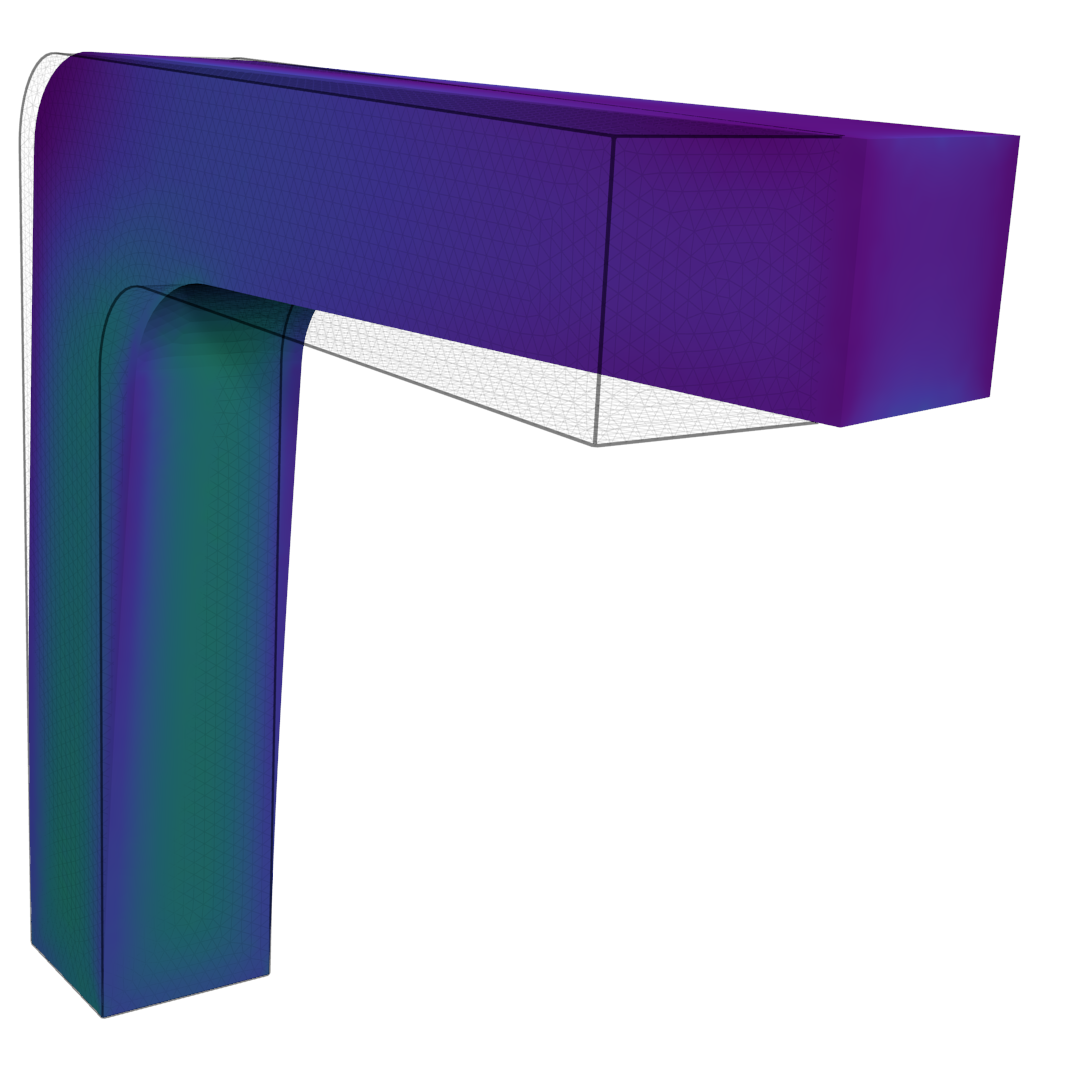
\includegraphics[width=0.305\figurewidth]{figures/hook2_deformation}%
    };

    \node[image, below=of image1] (image2)
    {
        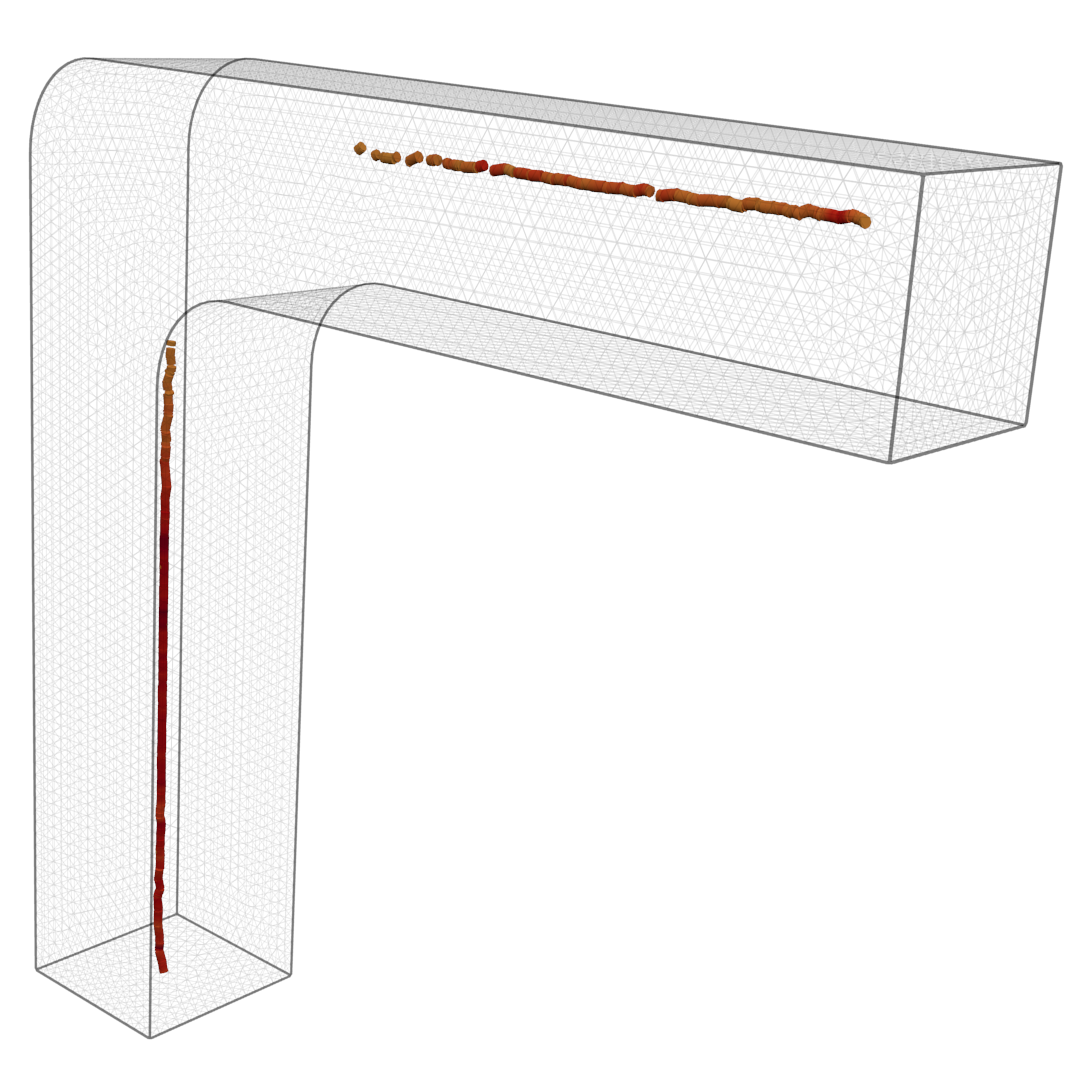
\includegraphics[width=0.305\figurewidth]{figures/hook2_lines}%
    };

    \node[image, below=of image2] (image3)
    {
        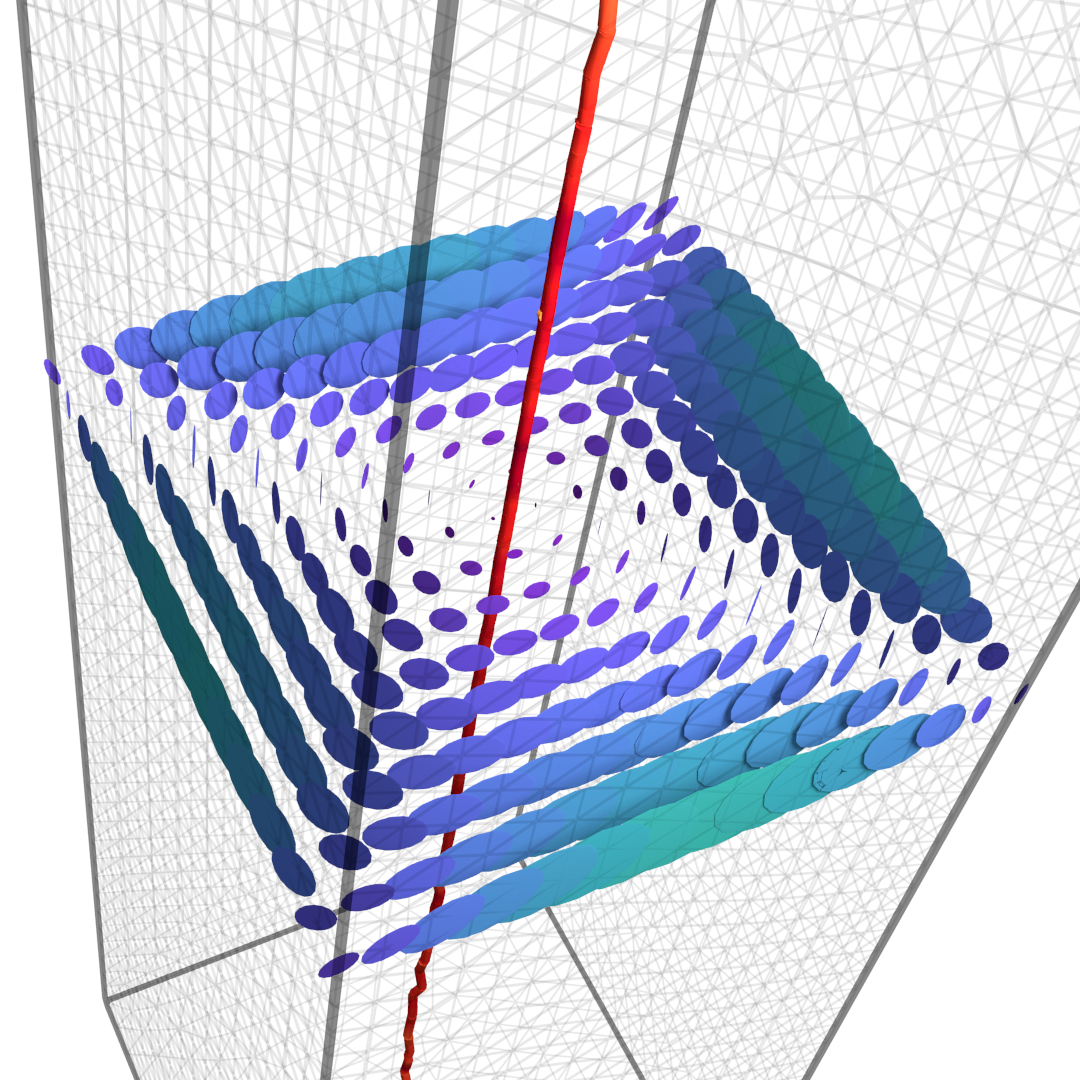
\includegraphics[width=0.305\figurewidth]{figures/hook2_detail1}%
    };

    \node[image, below=of image3] (image4)
    {
        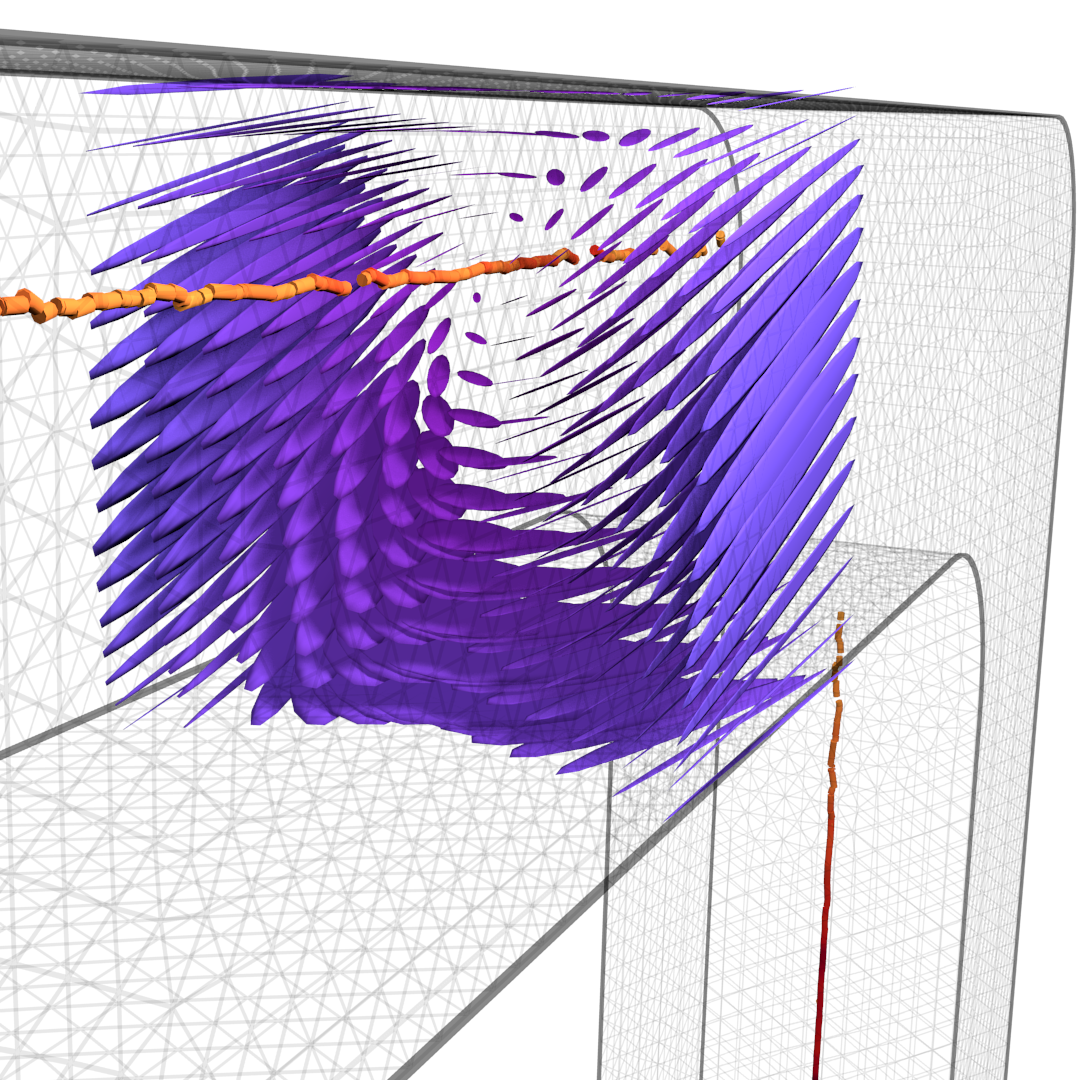
\includegraphics[width=0.305\figurewidth]{figures/hook2_detail2}%
    };

    \node[image, right=of image1] (image5)
    {
        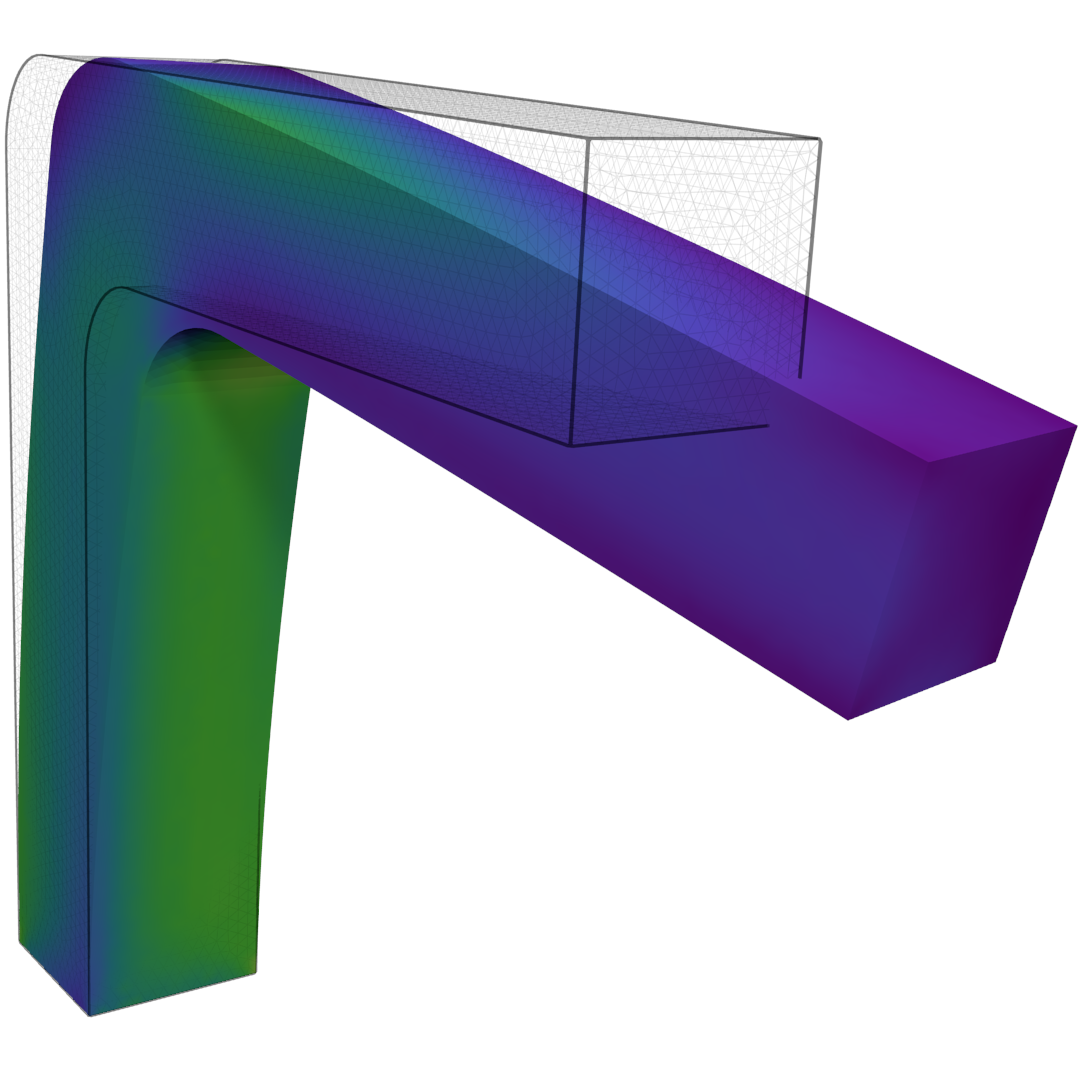
\includegraphics[width=0.305\figurewidth]{figures/hook3_deformation}%
    };

    \node[image, below=of image5] (image6)
    {
        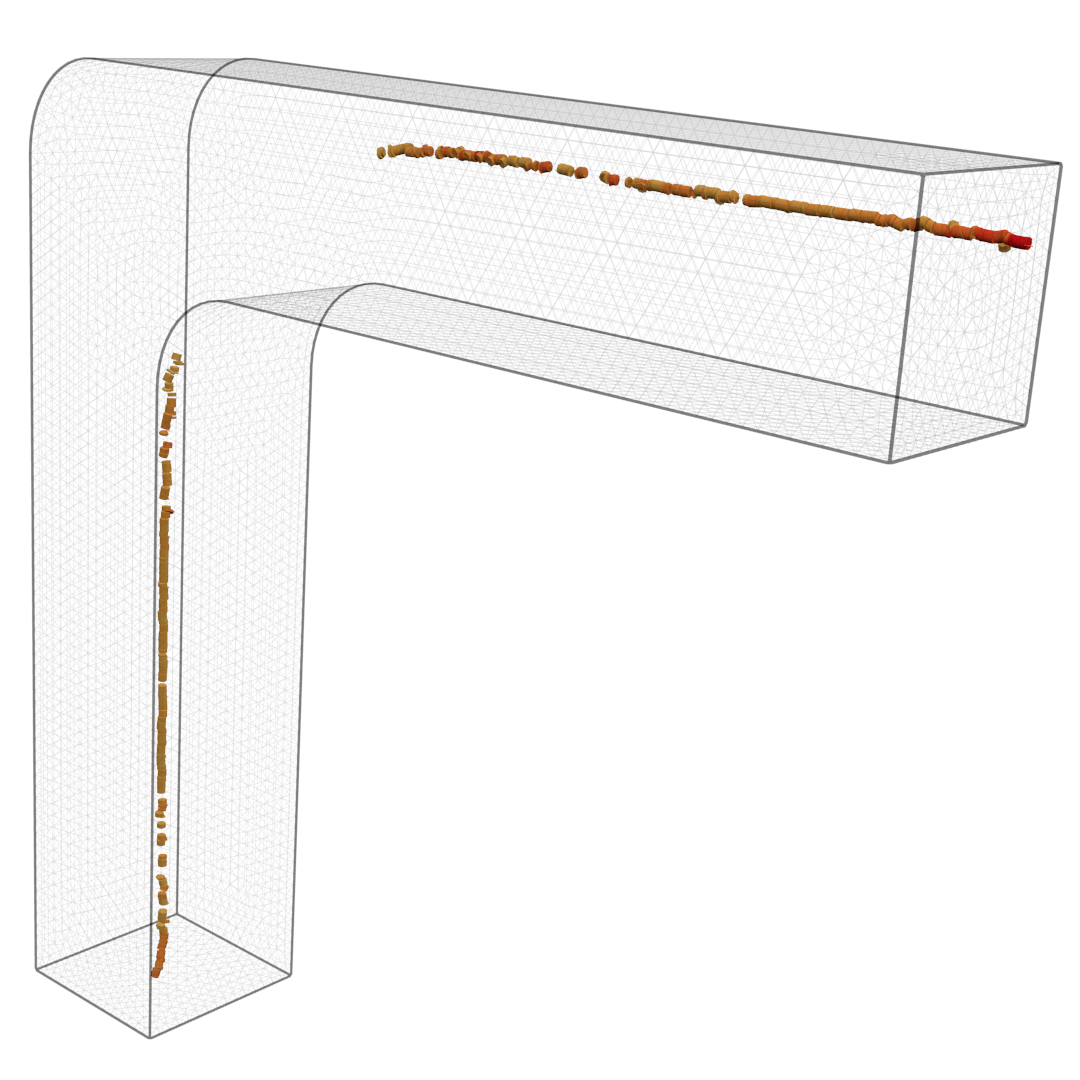
\includegraphics[width=0.305\figurewidth]{figures/hook3_lines}%
    };

    \node[image, below=of image6] (image7)
    {
        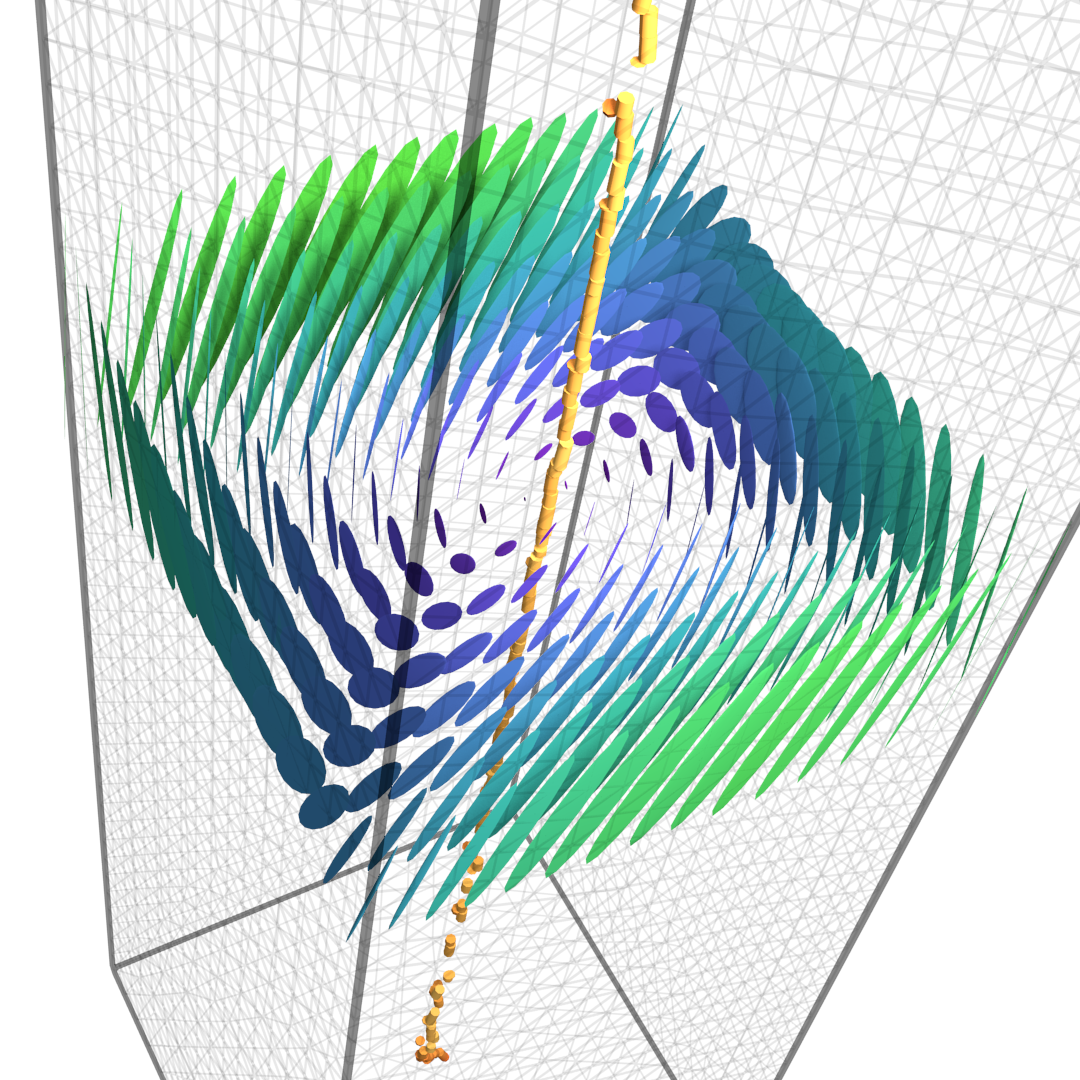
\includegraphics[width=0.305\figurewidth]{figures/hook3_detail1}%
    };

    \node[image, below=of image7] (image8)
    {
        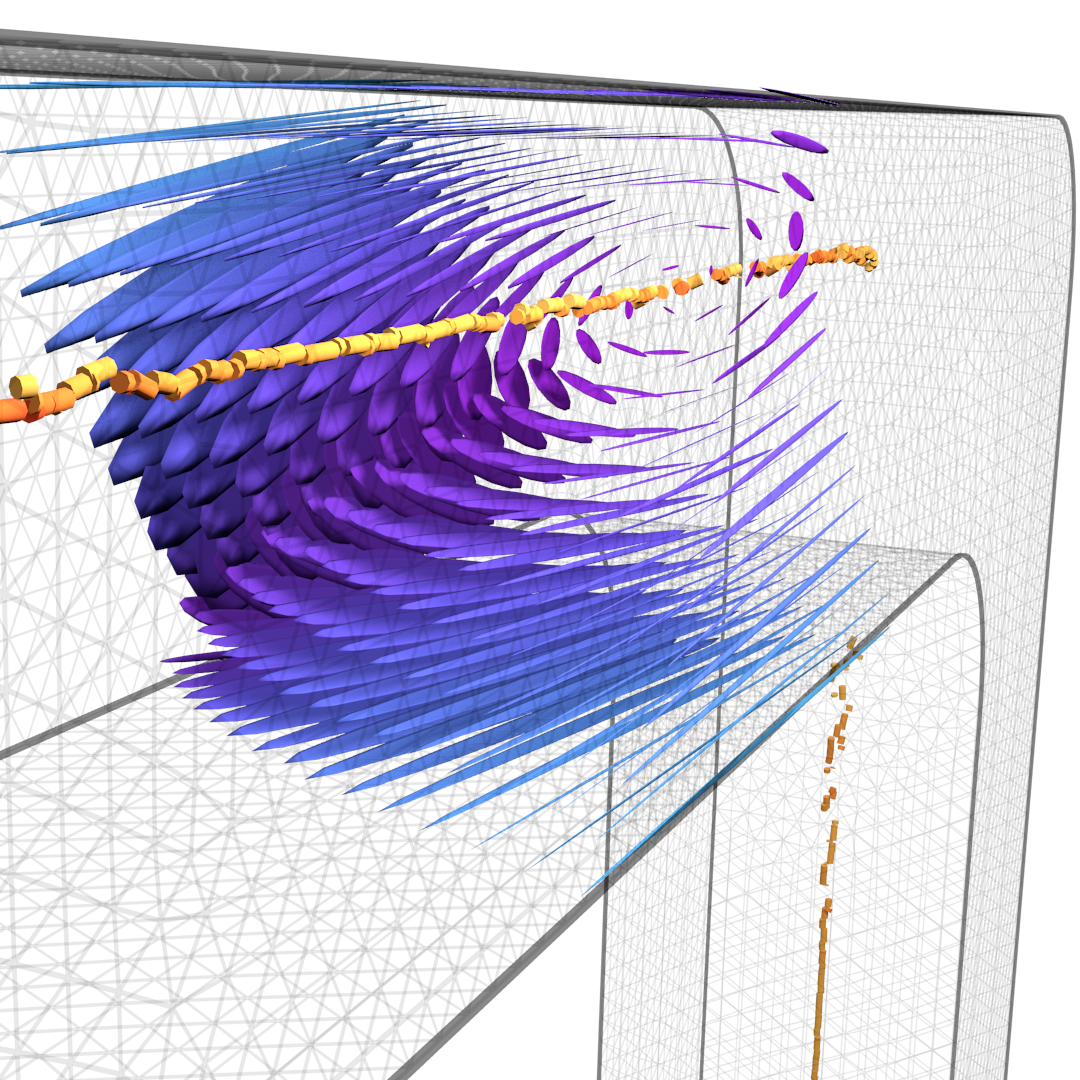
\includegraphics[width=0.305\figurewidth]{figures/hook3_detail2}%
    };

    % This is how you can add a color scale

    \node[anchor=south west, yshift=-4mm] (stabscale) at (image8.south east){
        \begin{axis}[
            scale only axis,
            height=2.8cm,
            hide axis,
            domain=1:20,
            colorbar,
            colorbar/width=0.25cm,
            colormap name={rdoryl},
            point meta min=-5, point meta max=11,
            colorbar style={
                title=$\log(s)$,
                scaled ticks=false,
                ytick={-5, 11}
            }]
        \end{axis}
    };
    \node[anchor=south west, xshift=1.3mm] at (stabscale.north west){
        \begin{axis}[
            scale only axis,
            height=2.8cm,
            hide axis,
            domain=1:20,
            colorbar,
            colorbar/width=0.25cm,
            colormap name={cubicyf},
            point meta min=0, point meta max=8e9,
            colorbar style={
                title=$\sigma_{\text{vM}}$,
                scaled ticks=false,
                ytick={0, 8e9}
            }]
        \end{axis}
    };

\end{tikzpicture}
    \caption{Tensor core lines for two different deformations in the
             \textsc{Handle} dataset. On the top, we show the resulting
             deformations. The von Mises stress $\sigma_{\textnormal{vM}}$ is
             color-coded on the surface. We represent the tensor core line as
             tubes in the undeformed coordinate system. Their color indicates
             the numerical stability $s$. The tensor field is shown for context
             using elliptical glyphs.}
    \label{fig:hooks}
\end{figure}
%
This case shows a handle-like structure with a right angle being deformed in
two different ways.
%
One end is fixed, while the other end experiences different displacements.
%
The first is a rotation around the shaft, which applies a torque to it.
%
The second includes an additional downward shift.
%
\Cref{fig:hooks} shows a tensor core line in the center of the shaft for both
cases.
%
Interestingly, a line is also visible in the ``handle''-part of the structure,
even though no direct torque was applied here.
%
The line in the handle shifts away from the plane of symmetry in the second
deformation case.
%
A look at the tensor field around the core lines confirms that they are indeed
the center of a swirling behavior of the tensor field.
%
% subsection hook (end)
%
\subsection{Truck Bumper} % (fold)
\label{sub:truck_bumper}
%
This case shows a load applied to the extreme end of the bumper of a cargo
truck.
%
Applying our algorithm to the dataset results in a large number of lines being
found all over the domain.
%
This may in part be explained by the low resolution of the simulation.
%
After applying a filter on the numeric stability $s$, two lines with high
stability stand out.
%
Somewhat counterintuitively, these are found on the side opposite to the end
experiencing the load.
%
In \cref{fig:truck_bumper}, we can clearly see the radial behavior of the
tensor field around both lines.
%
Finding these locations by manually inspecting the tensor field in detail would
be a tedious task.
%
Using the tensor core line extractor, they can be identified at a glance.
%
\begin{figure}[p]
    \centering
    \setlength\figurewidth\textwidth
    %
%
\pgfplotsset{colormap={cubicyf}{
rgb = (0.5151, 0.0482, 0.66969999999999996)
rgb = (0.52071100000000003, 0.16895499999999999, 0.80057400000000001)
rgb = (0.49369400000000002, 0.27859600000000001, 0.91182399999999997)
rgb = (0.44002599999999997, 0.369475, 0.98497800000000002)
rgb = (0.39893200000000001, 0.45759300000000003, 0.98705299999999996)
rgb = (0.35065099999999999, 0.54064400000000001, 0.92960799999999999)
rgb = (0.29882700000000001, 0.61562499999999998, 0.85772899999999996)
rgb = (0.239928, 0.68506100000000003, 0.76953099999999997)
rgb = (0.22883200000000001, 0.73934900000000003, 0.67328699999999997)
rgb = (0.263297, 0.78608, 0.56998800000000005)
rgb = (0.29810700000000001, 0.82833699999999999, 0.46021400000000001)
rgb = (0.33091999999999999, 0.86407100000000003, 0.35267399999999999)
rgb = (0.38306000000000001, 0.898169, 0.28730899999999998)
rgb = (0.49023, 0.91748099999999999, 0.30796099999999998)
rgb = (0.62372000000000005, 0.92602600000000002, 0.33230900000000002)
rgb = (0.71745800000000004, 0.92527000000000004, 0.342476)
rgb = (0.80000000000000004, 0.92549999999999999, 0.35289999999999999)
}}
\pgfplotsset{colormap={rdoryl}{
rgb(0)=(1, 1, 0.80000000000000004)
rgb(1)=(1, 0.96678200000000003, 0.71879999999999999)
rgb(2)=(1, 0.93134899999999998, 0.63218799999999997)
rgb(3)=(0.998139, 0.89219499999999996, 0.54929600000000001)
rgb(4)=(0.99617100000000003, 0.85282599999999997, 0.46662100000000001)
rgb(5)=(0.99607800000000002, 0.77780899999999997, 0.38394499999999998)
rgb(6)=(0.99607800000000002, 0.70103800000000005, 0.30126900000000001)
rgb(7)=(0.99418700000000004, 0.62805100000000003, 0.26777400000000001)
rgb(8)=(0.99221800000000004, 0.55521699999999996, 0.23627799999999999)
rgb(9)=(0.99024999999999996, 0.43280299999999999, 0.20096900000000001)
rgb(10)=(0.98828099999999997, 0.30878899999999998, 0.16553599999999999)
rgb(11)=(0.94017700000000004, 0.20592099999999999, 0.137793)
rgb(12)=(0.89096500000000001, 0.10356, 0.110235)
rgb(13)=(0.81656300000000004, 0.051580000000000001, 0.12918099999999999)
rgb(14)=(0.741761, 0.00040000000000000002, 0.148866)
rgb(15)=(0.62203799999999998, 0, 0.14902000000000001)
rgb(16)=(0.50196099999999999, 0, 0.14902000000000001)
}}
%
\begin{tikzpicture}
    \tikzstyle{image} = [inner sep=0, outer sep=0, node distance = 0 and 0]

    % place image in node
    \node[image] (image1)
    {
        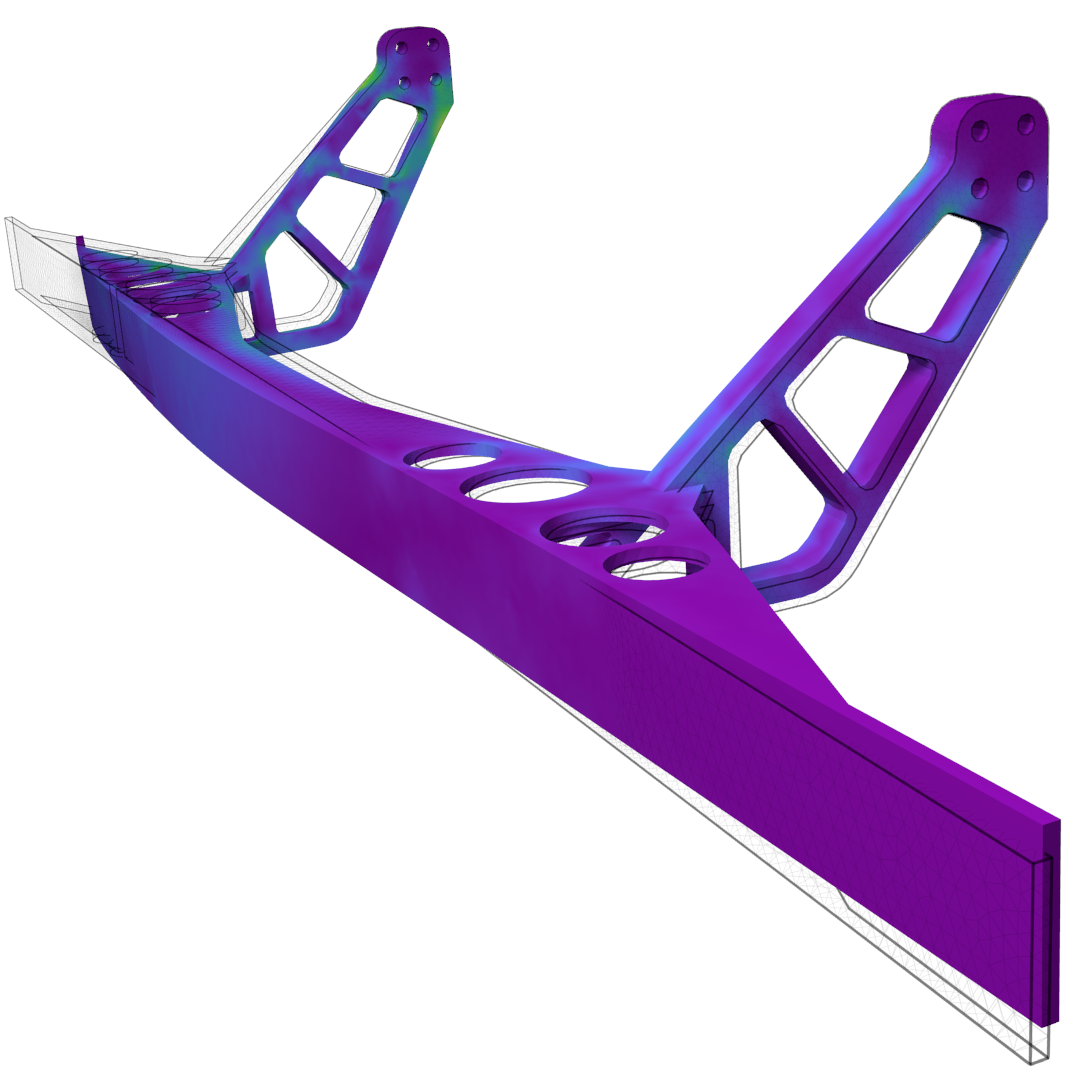
\includegraphics[width=0.22\figurewidth]{figures/truck_bumper_deformation}%
    };

    % place next image to the right with a little space in between
    \node[image, right=of image1, xshift=0.25cm] (image2)
    {
        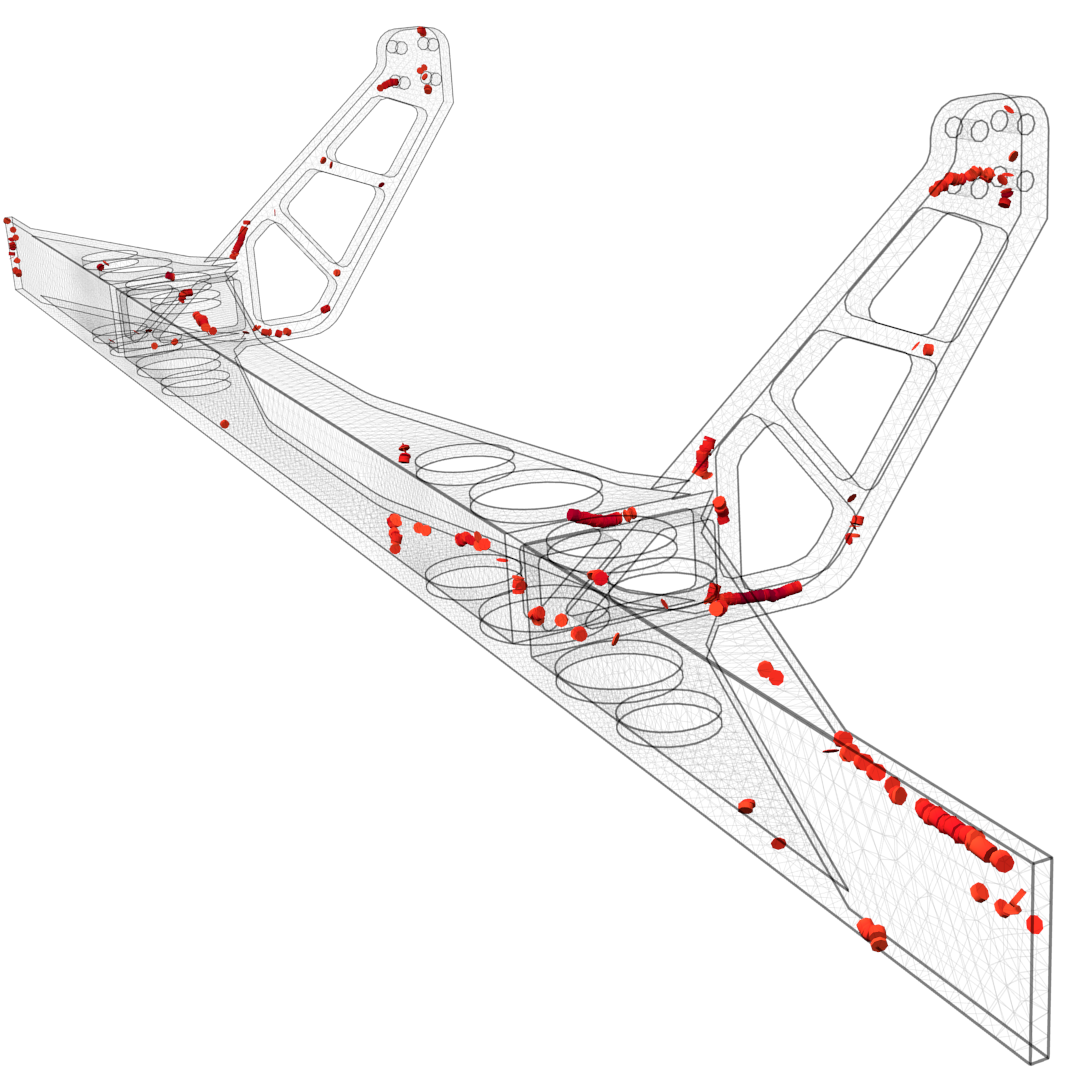
\includegraphics[width=0.22\figurewidth]{figures/truck_bumper_lines}%
    };
    % create new coordinate system on image2:
    \begin{scope}[
        shift=(image2.south west), % origin is lower left corner
        x={($(image2.south east)-(image2.south west)$)}, % x axis is lower side
        y={($(image2.north west)-(image2.south west)$)}] % y axis is left side
        % uncomment the following three lines to show a helper grid that helps
        % with finding coordinates
        % \draw[help lines,xstep=.1,ystep=.1] (0,0) grid (1,1);
        % \foreach \x in {0,1,...,9} { \node [anchor=north] at (\x/10,0) {\scriptsize 0.\x}; }
        % \foreach \y in {0,1,...,9} { \node [anchor=east] at (0,\y/10) {\scriptsize 0.\y}; }
        % draw stuff on image
        % (0, 0) is lower left corner, (1, 1) is upper right
        \draw [thin, -] (0.55, 0.535) -- (0.55, 0.6) node [anchor=south] {\large \textbf{$1$}};
        \draw [thin, -] (0.72, 0.435) -- (0.8, 0.4) node [anchor=west] {\large \textbf{$2$}};
    \end{scope}

    \node[image, right=of image2, xshift=0.25cm] (image3)
    {
        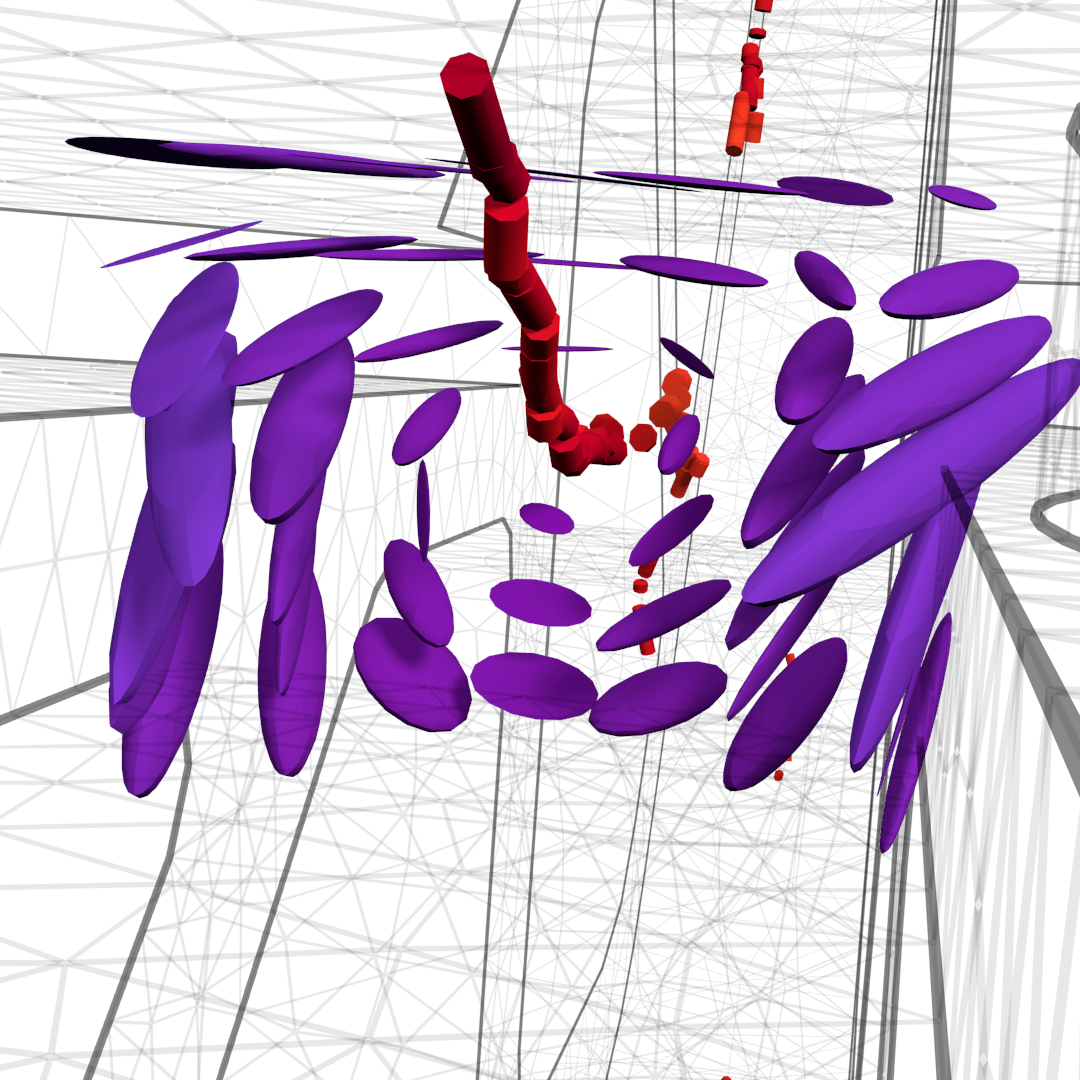
\includegraphics[width=0.22\figurewidth]{figures/truck_bumper_detail2}%
    };
    % place a text on the lower left corner of image3
    \node [anchor=south west] at (image3.south west) {\LARGE \textbf{$1$}};

    \node[image, right=of image3, xshift=0.25cm] (image4)
    {
        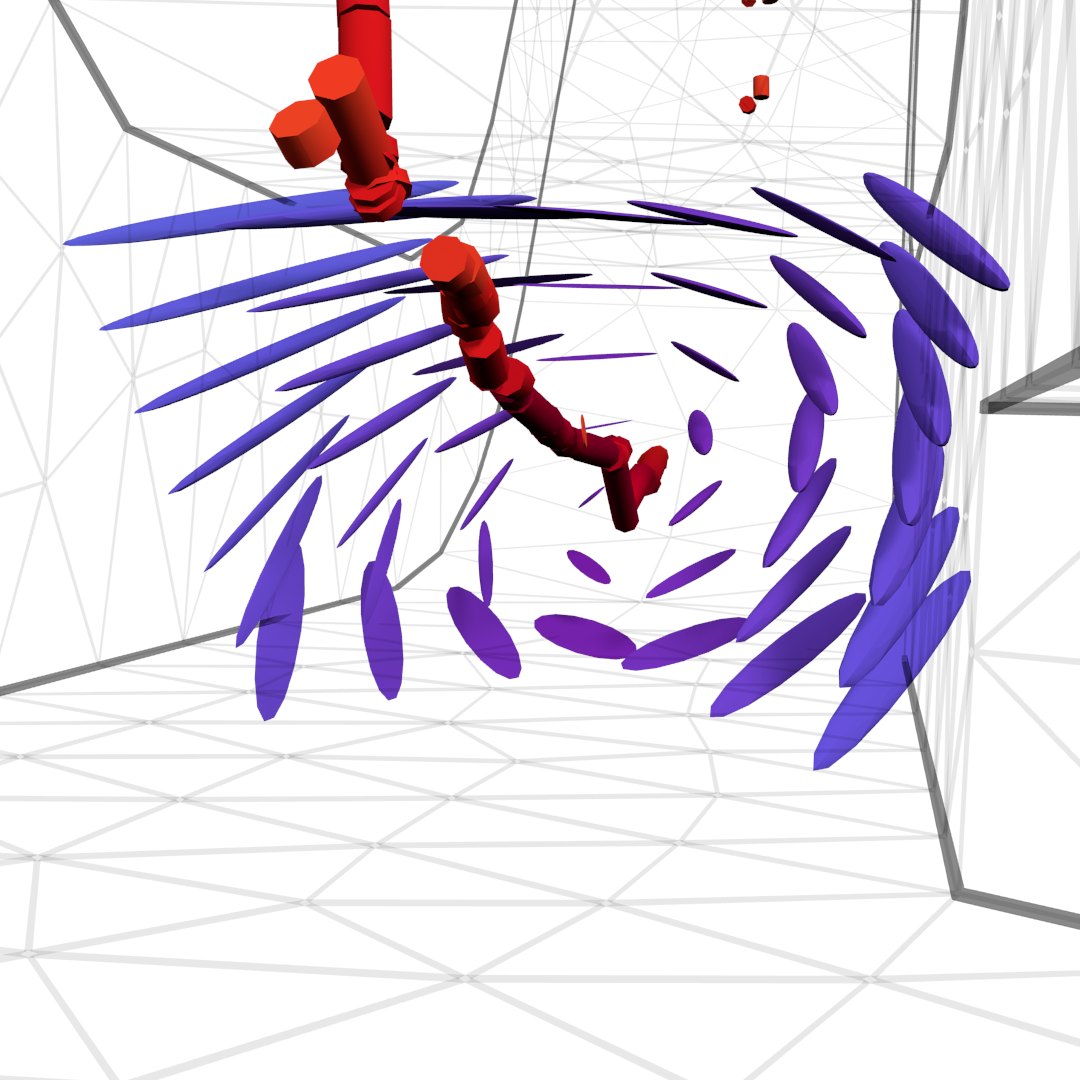
\includegraphics[width=0.22\figurewidth]{figures/truck_bumper_detail1}%
    };
    \node [anchor=south west] at (image4.south west) {\LARGE \textbf{$2$}};

    \node[anchor=north west, xshift=-0.7cm, yshift=0.15cm] at (image4.north east){
        \begin{axis}[
            scale only axis,
            height=1.1cm,
            hide axis,
            domain=1:20,
            colorbar,
            colorbar/width=0.25cm,
            colormap name={cubicyf},
            point meta min=0, point meta max=9e6,
            colorbar style={
                title=$\sigma_{\text{vM}}$,
                scaled ticks=false,
                ytick={0, 9e6}
            }]
        \end{axis}
    };
    \node[anchor=south west, xshift=-0.8cm, yshift=-0.15cm] at (image4.south east){
        \begin{axis}[
            scale only axis,
            height=1.1cm,
            hide axis,
            domain=1:20,
            colorbar,
            colorbar/width=0.25cm,
            colormap name={rdoryl},
            point meta min=1.5, point meta max=15,
            colorbar style={
                title=$\log(s)$,
                scaled ticks=false,
                ytick={1.5, 15}
            }]
        \end{axis}
    };

\end{tikzpicture}
    \vspace*{-5mm}
    \caption{Tensor core lines in the \textsc{truck bumper} dataset. The
             deformation shown on the top left is scaled by a factor of
             \num{500} for illustrative purposes. The bottom shows detail views
             of two interesting lines with tensor glyphs for context.}
    \label{fig:truck_bumper}
\end{figure}
%
% subsection truck_bumper (end)
%
\subsection{Crane} % (fold)
\label{sub:crane}
%
In this dataset, the arm of a crane is exposed to a downward pull applied to
the lower side of a cube at the end (see \cref{fig:crane}).
%
Similar to the truck bumper, it is not intuitively clear in which parts of the
structure a swirling behavior of the tensors will occur, just from looking at
the setup of the case.
%
Almost all stable solutions we find are located in the diagonal rods on the
lower side.
%
Again, looking closely at the tensors around the core lines, we can see the
radial behavior.
%
\begin{figure}[p]
    \centering
    \setlength\figurewidth\linewidth
    %
%
\pgfplotsset{colormap={cubicyf}{
rgb = (0.5151, 0.0482, 0.66969999999999996)
rgb = (0.52071100000000003, 0.16895499999999999, 0.80057400000000001)
rgb = (0.49369400000000002, 0.27859600000000001, 0.91182399999999997)
rgb = (0.44002599999999997, 0.369475, 0.98497800000000002)
rgb = (0.39893200000000001, 0.45759300000000003, 0.98705299999999996)
rgb = (0.35065099999999999, 0.54064400000000001, 0.92960799999999999)
rgb = (0.29882700000000001, 0.61562499999999998, 0.85772899999999996)
rgb = (0.239928, 0.68506100000000003, 0.76953099999999997)
rgb = (0.22883200000000001, 0.73934900000000003, 0.67328699999999997)
rgb = (0.263297, 0.78608, 0.56998800000000005)
rgb = (0.29810700000000001, 0.82833699999999999, 0.46021400000000001)
rgb = (0.33091999999999999, 0.86407100000000003, 0.35267399999999999)
rgb = (0.38306000000000001, 0.898169, 0.28730899999999998)
rgb = (0.49023, 0.91748099999999999, 0.30796099999999998)
rgb = (0.62372000000000005, 0.92602600000000002, 0.33230900000000002)
rgb = (0.71745800000000004, 0.92527000000000004, 0.342476)
rgb = (0.80000000000000004, 0.92549999999999999, 0.35289999999999999)
}}
\pgfplotsset{colormap={rdoryl}{
rgb(0)=(1, 1, 0.80000000000000004)
rgb(1)=(1, 0.96678200000000003, 0.71879999999999999)
rgb(2)=(1, 0.93134899999999998, 0.63218799999999997)
rgb(3)=(0.998139, 0.89219499999999996, 0.54929600000000001)
rgb(4)=(0.99617100000000003, 0.85282599999999997, 0.46662100000000001)
rgb(5)=(0.99607800000000002, 0.77780899999999997, 0.38394499999999998)
rgb(6)=(0.99607800000000002, 0.70103800000000005, 0.30126900000000001)
rgb(7)=(0.99418700000000004, 0.62805100000000003, 0.26777400000000001)
rgb(8)=(0.99221800000000004, 0.55521699999999996, 0.23627799999999999)
rgb(9)=(0.99024999999999996, 0.43280299999999999, 0.20096900000000001)
rgb(10)=(0.98828099999999997, 0.30878899999999998, 0.16553599999999999)
rgb(11)=(0.94017700000000004, 0.20592099999999999, 0.137793)
rgb(12)=(0.89096500000000001, 0.10356, 0.110235)
rgb(13)=(0.81656300000000004, 0.051580000000000001, 0.12918099999999999)
rgb(14)=(0.741761, 0.00040000000000000002, 0.148866)
rgb(15)=(0.62203799999999998, 0, 0.14902000000000001)
rgb(16)=(0.50196099999999999, 0, 0.14902000000000001)
}}
%
\begin{tikzpicture}[
    font=\small
]
    \tikzstyle{image} = [inner sep=0, outer sep=0, node distance = 0 and 0]

    % place image in node
    \node[image] (image1)
    {
        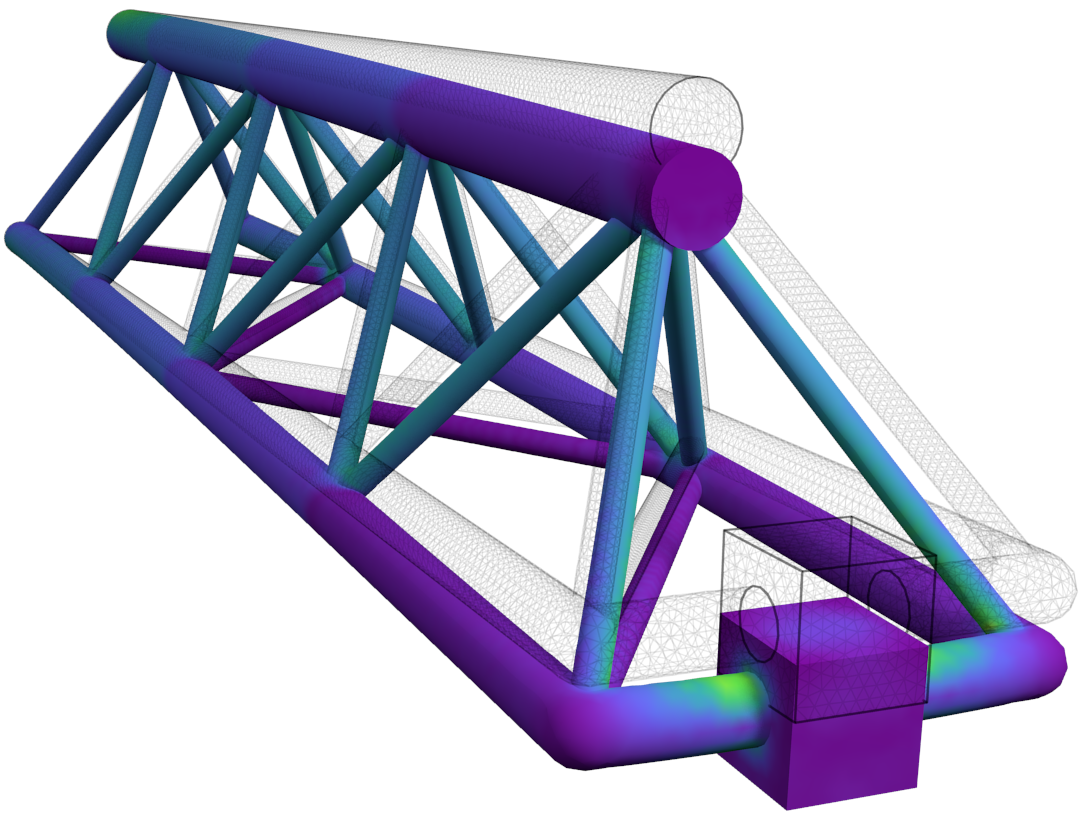
\includegraphics[width=0.333\figurewidth]{figures/crane_deformation}%
    };

    % place next image to the right with a little space in between
    \node[image, right=of image1] (image2)
    {
        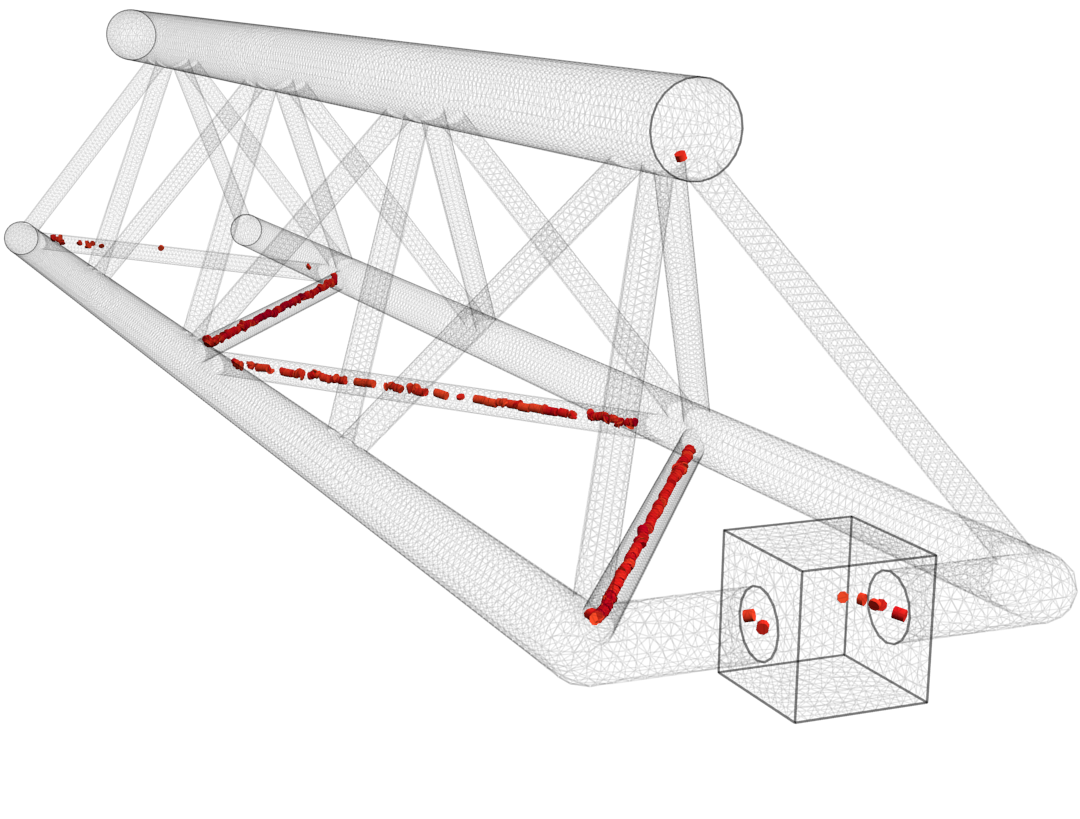
\includegraphics[width=0.333\figurewidth]{figures/crane_lines}%
    };

    \node[image, right=of image2] (image3)
    {
        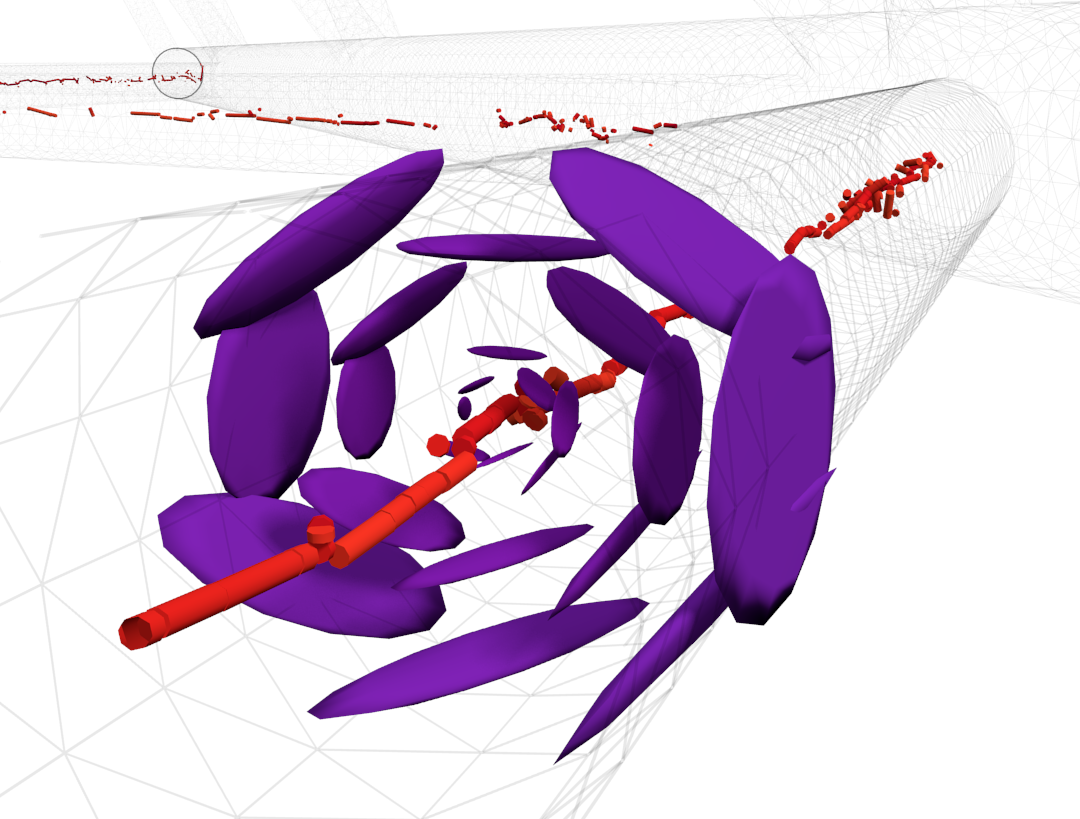
\includegraphics[width=0.333\figurewidth]{figures/crane_detail}%
    };

    \node[anchor=north east] at (image2.south){
        \begin{axis}[
            scale only axis,
            height=2.8cm,
            hide axis,
            domain=1:20,
            colorbar horizontal,
            colorbar/width=0.25cm,
            colormap name={cubicyf},
            point meta min=0, point meta max=1.5e6,
            colorbar style={
                title=\strut$\sigma_{\textnormal{vM}}$,
                scaled ticks=false,
                xtick={0, 1.5e6}
            }]
        \end{axis}
    };
    \node[anchor=north west] at (image2.south){
        \begin{axis}[
            scale only axis,
            height=2.8cm,
            hide axis,
            domain=1:20,
            colorbar horizontal,
            colorbar/width=0.25cm,
            colormap name={rdoryl},
            point meta min=-7.5, point meta max=11,
            colorbar style={
                title=\strut$\log(s)$,
                scaled ticks=false,
                xtick={-7.5, 11}
            }]
        \end{axis}
    };

\end{tikzpicture}
    \vspace*{-7mm}
    \caption{Tensor core lines in the \textsc{Crane} dataset. The resulting
             deformation on the left is scaled by a factor of
             \num{1500}.}
    \label{fig:crane}
\end{figure}
%
% subsection crane (end)
%
\subsection{Spring} % (fold)
\label{sub:spring}
%
A simulation of a coil spring being compressed and slightly bent between two
plates is shown in~\cref{fig:spring}.
%
Apart from numerical noise in the poorly resolved plates, we find significant
tensor core lines at the center of the coil's cross-section.
%
A look at the tensor field visualized by glyphs reveals that in this case, we
do not have a simple swirling behavior of the tensors.
%
Instead, the tensor field shows something similar to a hyperbolic behavior in
vector fields.
%
In the rightmost picture in~\cref{fig:spring}, we can see that eigenvector
trajectories start at the wall on both sides and curve into the same direction.
%
This direction is reversed on the top and bottom side of the spring.
%
In the middle, there is a surface where these curves become straight lines along
the diameter of the cross-section.
%
This is exactly where we find a tensor core line.
%
\begin{figure}[p]
    \centering
    \setlength\figurewidth\linewidth
    %
%
\pgfplotsset{colormap={cubicyf}{
rgb = (0.5151, 0.0482, 0.66969999999999996)
rgb = (0.52071100000000003, 0.16895499999999999, 0.80057400000000001)
rgb = (0.49369400000000002, 0.27859600000000001, 0.91182399999999997)
rgb = (0.44002599999999997, 0.369475, 0.98497800000000002)
rgb = (0.39893200000000001, 0.45759300000000003, 0.98705299999999996)
rgb = (0.35065099999999999, 0.54064400000000001, 0.92960799999999999)
rgb = (0.29882700000000001, 0.61562499999999998, 0.85772899999999996)
rgb = (0.239928, 0.68506100000000003, 0.76953099999999997)
rgb = (0.22883200000000001, 0.73934900000000003, 0.67328699999999997)
rgb = (0.263297, 0.78608, 0.56998800000000005)
rgb = (0.29810700000000001, 0.82833699999999999, 0.46021400000000001)
rgb = (0.33091999999999999, 0.86407100000000003, 0.35267399999999999)
rgb = (0.38306000000000001, 0.898169, 0.28730899999999998)
rgb = (0.49023, 0.91748099999999999, 0.30796099999999998)
rgb = (0.62372000000000005, 0.92602600000000002, 0.33230900000000002)
rgb = (0.71745800000000004, 0.92527000000000004, 0.342476)
rgb = (0.80000000000000004, 0.92549999999999999, 0.35289999999999999)
}}
\pgfplotsset{colormap={rdoryl}{
rgb(0)=(1, 1, 0.80000000000000004)
rgb(1)=(1, 0.96678200000000003, 0.71879999999999999)
rgb(2)=(1, 0.93134899999999998, 0.63218799999999997)
rgb(3)=(0.998139, 0.89219499999999996, 0.54929600000000001)
rgb(4)=(0.99617100000000003, 0.85282599999999997, 0.46662100000000001)
rgb(5)=(0.99607800000000002, 0.77780899999999997, 0.38394499999999998)
rgb(6)=(0.99607800000000002, 0.70103800000000005, 0.30126900000000001)
rgb(7)=(0.99418700000000004, 0.62805100000000003, 0.26777400000000001)
rgb(8)=(0.99221800000000004, 0.55521699999999996, 0.23627799999999999)
rgb(9)=(0.99024999999999996, 0.43280299999999999, 0.20096900000000001)
rgb(10)=(0.98828099999999997, 0.30878899999999998, 0.16553599999999999)
rgb(11)=(0.94017700000000004, 0.20592099999999999, 0.137793)
rgb(12)=(0.89096500000000001, 0.10356, 0.110235)
rgb(13)=(0.81656300000000004, 0.051580000000000001, 0.12918099999999999)
rgb(14)=(0.741761, 0.00040000000000000002, 0.148866)
rgb(15)=(0.62203799999999998, 0, 0.14902000000000001)
rgb(16)=(0.50196099999999999, 0, 0.14902000000000001)
}}
%
\begin{tikzpicture}[
    font=\small
]
    \tikzstyle{image} = [inner sep=0, outer sep=0, node distance = 0 and 0]

    \node[image] (image1)
    {
        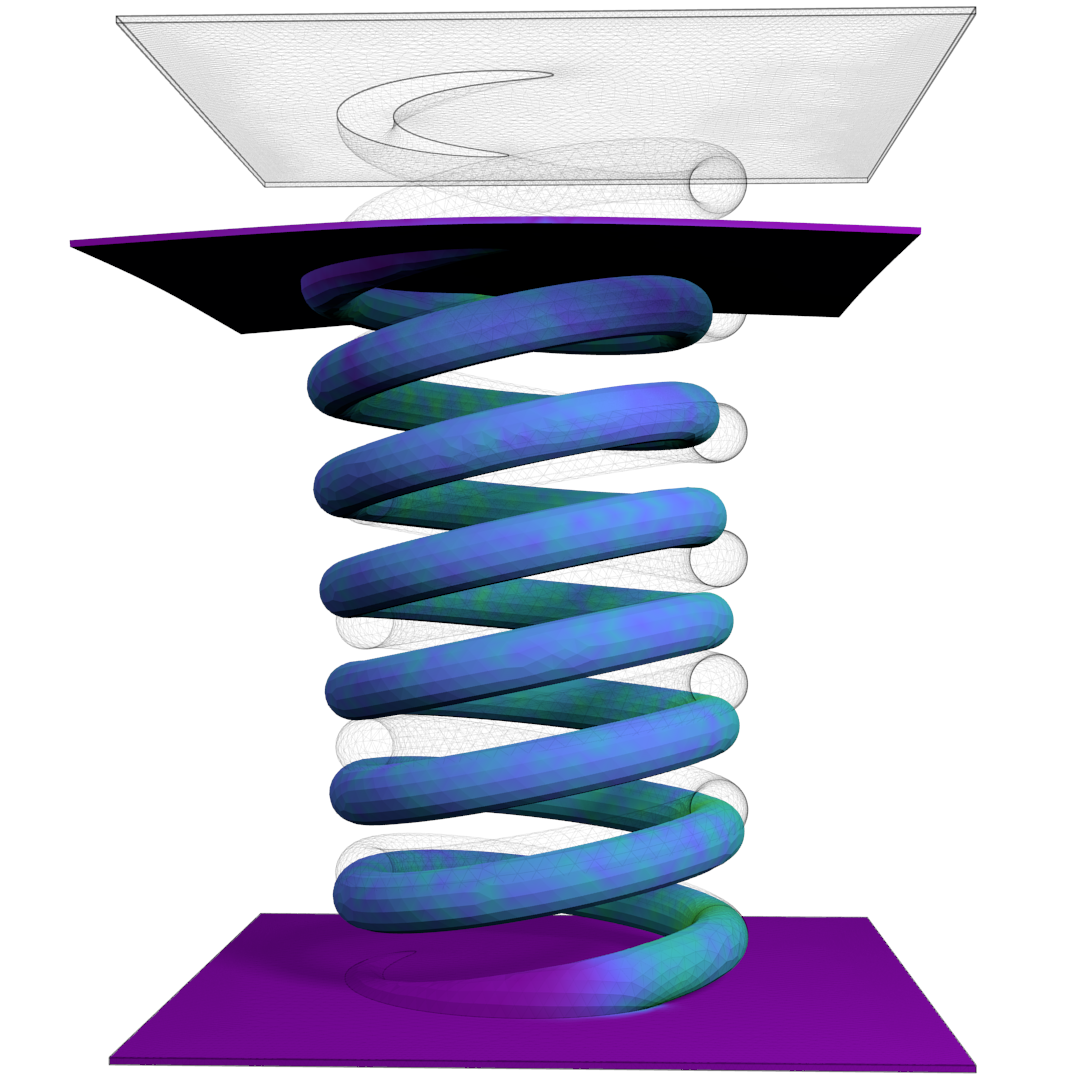
\includegraphics[width=0.22\figurewidth]{figures/spring_deformation}%
    };

    \node[image, right=of image1, xshift=0.25cm] (image2)
    {
        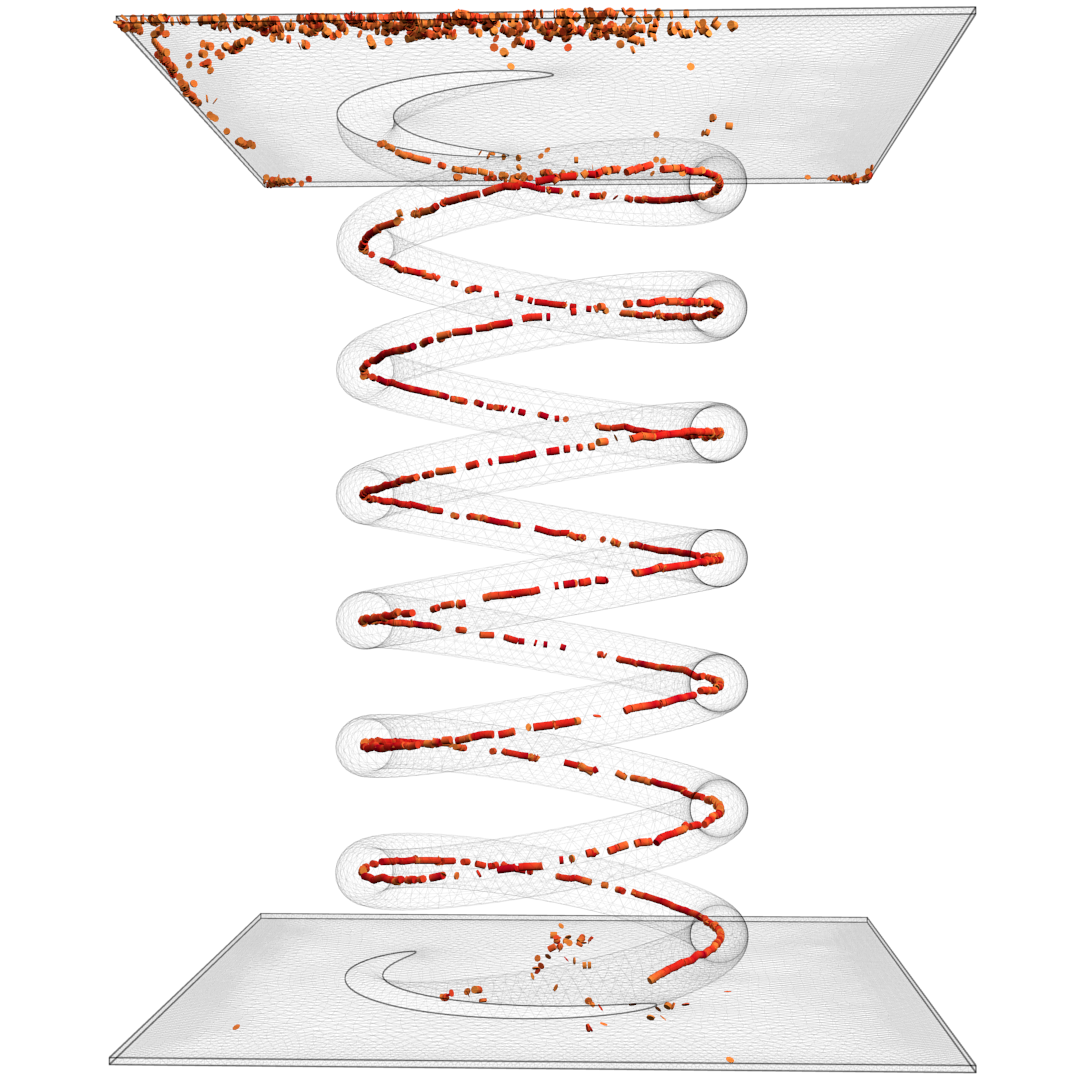
\includegraphics[width=0.22\figurewidth]{figures/spring_lines}%
    };

    \node[image, right=of image2, xshift=0.25cm] (image3)
    {
        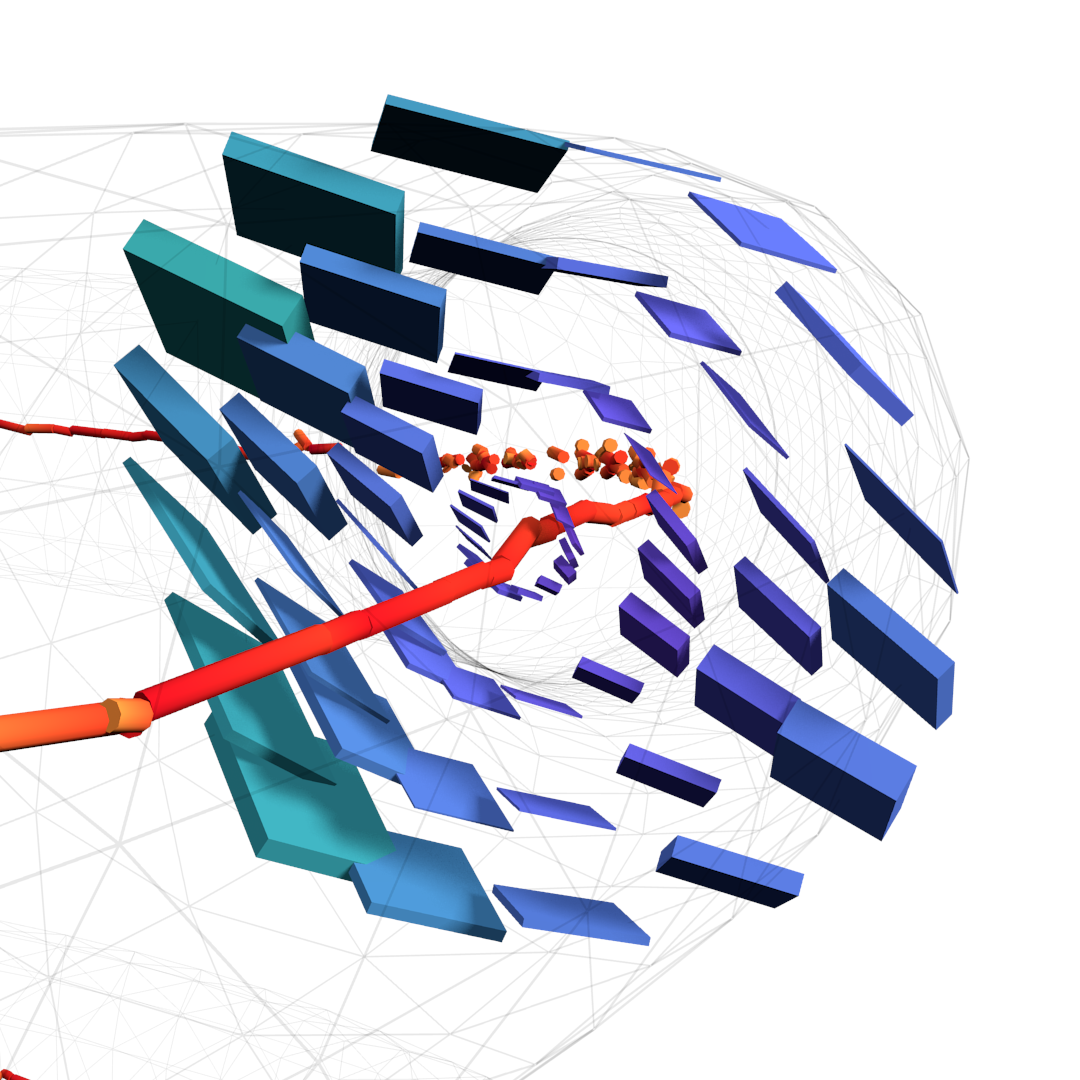
\includegraphics[width=0.22\figurewidth]{figures/spring_detail1_box}%
    };

    \node[image, right=of image3, xshift=0.25cm] (image4)
    {
        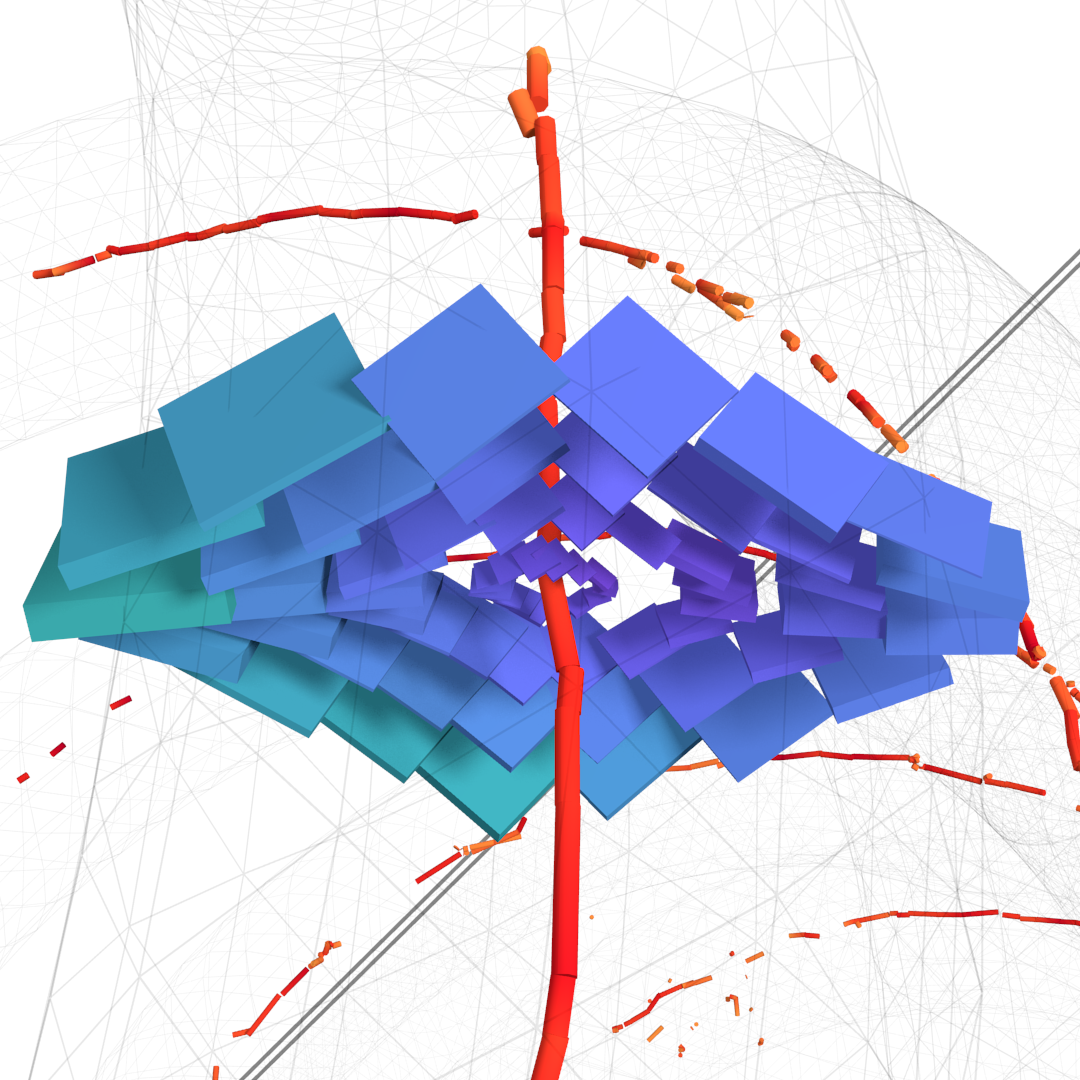
\includegraphics[width=0.22\figurewidth]{figures/spring_detail2_box}%
    };

    \node[anchor=north west, xshift=-0.7cm, yshift=0.15cm] at (image4.north east){
        \begin{axis}[
            scale only axis,
            height=1.1cm,
            hide axis,
            domain=1:20,
            colorbar,
            colorbar/width=0.25cm,
            colormap name={cubicyf},
            point meta min=0, point meta max=1e9,
            colorbar style={
                title=$\sigma_{\text{vM}}$,
                scaled ticks=false,
                ytick={0, 1e9}
            }]
        \end{axis}
    };
    \node[anchor=south west, xshift=-0.8cm, yshift=-0.15cm] at (image4.south east){
        \begin{axis}[
            scale only axis,
            height=1.1cm,
            hide axis,
            domain=1:20,
            colorbar,
            colorbar/width=0.25cm,
            colormap name={rdoryl},
            point meta min=3, point meta max=17,
            colorbar style={
                title=$\log(s)$,
                scaled ticks=false,
                ytick={3, 17}
            }]
        \end{axis}
    };

\end{tikzpicture}
    \vspace*{-5mm}
    \caption{Tensor core lines in the \textsc{Spring} dataset. We visualize the
             tensors near the core line with box glyphs in this case. They make
             it easier to see the hyperbolic behavior of the eigenvectors that
             occurs in the coil's cross-section. }
    \label{fig:spring}
\end{figure}
%
% subsection spring (end)
%
\subsection{Performance and Parameter Study} % (fold)
\label{sub:performance}
%
\begin{table}[p]
    \centering
    \caption{Performance of the algorithm for the datasets presented in this paper.}
    \begin{tabular}{lSSS}
        \toprule
        Dataset & {\# of cells/\num{e3}} & {time/\si{\second}} & {avg. time per face/\si{\milli\second}} \\% & avg. time/face (single core) [ms] \\
        \midrule
        \textsc{Cylinder} & 65 & 8 & 0.034 \\% & 0.14 \\
        \textsc{Handle} & 235 & 36 & 0.038 \\% & 0.16 \\
        \textsc{Truck Bumper} & 97 & 32 & 0.081 \\% & 0.36 \\
        \textsc{Crane} & 108 & 63 & 0.146 \\% & 0.59 \\
        \textsc{Spring} & 181 & 82 & 0.114 \\
        \bottomrule
    \end{tabular}\label{tab:performance}
\end{table}
%
The performance of our algorithm is dependent on the dataset.
%
If we find a large number of tensor core lines in the dataset, computation
will be slower as fewer cells can be discarded early.
%
We tested our algorithm using a consumer PC with a 4-core Intel Core i7 \ac{CPU}
at \SI{3.4}{\giga\hertz}.
%
Our implementation is parallelized over the faces of the dataset using
OpenMP~\cite{OMP2013}.
%
Performance numbers for the different datasets shown in this paper are presented
in \cref{tab:performance}.
%
To examine the dependence of the performance and results of our algorithm on the
parameters $M$, $\varepsilon_{\mathrm{t}}$ and $\varepsilon_{\mathrm{c}}$, we
conducted a parameter study.
%
We selected baseline parameters $M = 10^3$, $\varepsilon_{\mathrm{t}} =
\num{e-6}$ and $\varepsilon_{\mathrm{c}} = \num{e-3}$.
%
We then varied each parameter separately and applied our algorithm to the
cylinder dataset.
%
The results can be seen in \cref{fig:parameter_study}.
%
We can see that the performance is controlled by the threshold $M$, which
controls at which point we assume we are not converging onto an isolated
solution.
%
Increasing $M$ also increases the number of solutions we find.
%
However, if we look at the number of solutions that remain after filtering based
on numeric stability, it becomes clear that these solutions are only caused by
noise.
%
Increasing $M$ did not result in any additional numerically stable lines.
%
The parameters $\varepsilon_{\mathrm{t}}$ and $\varepsilon_{\mathrm{c}}$ have
almost no noticeable impact on runtime or solutions, unless we choose
unreasonable numbers.
%
In case of $\varepsilon_{\mathrm{t}}$, choosing a value that is larger than
\num{e-3} causes an explosion of the number of found solutions, as the
tolerance is not tight enough.
%
Choosing $\varepsilon_{\mathrm{c}}$ smaller than $\varepsilon_{\mathrm{t}}$
means that candidate solutions belonging to the same cluster often can not be
clustered, because the search radius is smaller than the distance between the
triangle centers.
%
Otherwise, $\varepsilon_{\mathrm{c}}$ is very stable.
%
This is because for solutions which are isolated points and belong to different
eigenvectors, the separation between clusters in direction space is rather
large.
%%
This means the choice of $\varepsilon_{\mathrm{c}}$ is not critical as
long as it is not chosen extremely small, or so large that solutions
which belong to different eigenvectors are clustered together.
%%

%
Stability tests on our other datasets all produced very similar results.
%
We recommend choosing $M = \num{e2}$, $\varepsilon_{\mathrm{t}} = \num{e-3}$ and
$\varepsilon_{\mathrm{c}} = \num{e-2}$ if performance is important.
%
If accuracy is important, we found that choosing stricter tolerances than $M =
\num{e3}$, $\varepsilon_{\mathrm{t}} = \num{e-6}$ and $\varepsilon_{\mathrm{c}}
= \num{e-3}$ does not produce noticeably better results.
%
\begin{figure}[t]
    \centering
    \tikzset{external/export=false}
    %
%
\definecolor{yellowdraw}{rgb}{0.996078, 0.701038, 0.301269}
% \definecolor{yellowdraw}{HTML}{E68600}
\definecolor{yellowfill}{HTML}{FFDDAC}
%
\begin{tikzpicture}
\pgfplotsset{myBar/.style={
	% small,
	width=3.5cm,
	ybar=1pt,
	% x = 12pt,
	bar width=9pt,
	bar shift=0pt,
	ytick align=outside,
	xtick style={draw=none},
	xtick = data,
	x tick label style={rotate=45,anchor=north east, yshift=0.18cm, xshift=0.2cm},
	axis x line*=bottom,
	enlarge x limits=0.15,
	after end axis/.code={ % Draw line indicating break
            \draw [ultra thick, white, decoration={snake, amplitude=1pt}, decorate] (rel axis cs:-0.01,1.05) -- (rel axis cs:1.01,1.05);
        },
    clip=false
}}
\begin{axis}[
	myBar,
	name = m_time,
	ymin=0,
	ymax=15.4,
	% xlabel=$M$,
	ylabel={run time [\si{\second}]},
	symbolic x coords = {$10$, $10^2$, $10^3$, $10^4$},
	axis y line*=left
]
\addplot[mycolor1, fill=mycolor1]
	coordinates {($10$,5) ($10^2$,6) ($10^3$,8.4) ($10^4$,15.4)};
\label{plt:runtime}
\end{axis}
%
\begin{axis}[
	myBar,
	name = eps_t_time,
	at = {(m_time.east)},
	xshift = 0.75cm,
	anchor = west,
	ymin=0,
	ymax=15.4,
	% xlabel=$\epsilon_t$,
	symbolic x coords = {$10^{-2}$, $10^{-3}$, $10^{-6}$, $10^{-9}$},
	hide y axis,
]
\addplot[mycolor1, fill=mycolor1]
	coordinates {($10^{-2}$,8.0) ($10^{-3}$,8.2) ($10^{-6}$,8.4) ($10^{-9}$,8.6)};
\end{axis}
%
\begin{axis}[
	myBar,
	name = eps_c_time,
	at = {(eps_t_time.east)},
	xshift = 0.75cm,
	anchor = west,
	ymin=0,
	ymax=15.4,
	% xlabel=$\epsilon_c$,
	symbolic x coords = {$10^{-2}$, $10^{-3}$, $10^{-6}$, $10^{-9}$},
	hide y axis,
]
\addplot[mycolor1, fill=mycolor1]
	coordinates {($10^{-2}$,8.4) ($10^{-3}$,8.4) ($10^{-6}$,8.4) ($10^{-9}$,8.4)};
\end{axis}
%
\begin{axis}[
	myBar,
	name = m_lines,
	at = {(m_time.below south west)},
	yshift = -1cm,
	anchor = north west,
	ymin=0,
	ymax=1100,
	ylabel = {\# lines},
	restrict y to domain*={0:1300},
	xlabel=$M$,
	symbolic x coords = {$10$, $10^{2}$, $10^{3}$, $10^{4}$},
	axis y line*=left
]
\addplot[yellowdraw,fill=yellowdraw]
	coordinates {($10$,0) ($10^{2}$,186) ($10^{3}$,440) ($10^{4}$,693)};
\label{plt:total_lines}
\addplot[mycolor4, fill=mycolor4]
	coordinates {($10$,0) ($10^{2}$,159) ($10^{3}$,153) ($10^{4}$,153)};
\label{plt:filtered_lines}
\end{axis}
%
\begin{axis}[
	myBar,
	name = eps_t_lines,
	at = {(m_lines.east)},
	xshift = 0.75cm,
	anchor = west,
	ymin=0,
	ymax=1100,
	restrict y to domain*={0:1300},
	xlabel=$\epsilon_t$,
	symbolic x coords = {$10^{-2}$, $10^{-3}$, $10^{-6}$, $10^{-9}$},
	hide y axis,
]
\addplot[yellowdraw,fill=yellowdraw]
	coordinates {($10^{-2}$,9000) ($10^{-3}$,455) ($10^{-6}$,440) ($10^{-9}$,435)};
\addplot[mycolor4, fill=mycolor4]
	coordinates {($10^{-2}$,156) ($10^{-3}$,153) ($10^{-6}$,153) ($10^{-9}$,153)};
\node[above] at (axis cs:$10^{-2}$,1300) {\textcolor{yellowdraw}{\small $9000$}};
\end{axis}
%
\begin{axis}[
	myBar,
	name = eps_c_lines,
	at = {(eps_t_lines.east)},
	xshift = 0.75cm,
	anchor = west,
	ymin=0,
	ymax=1100,
	restrict y to domain*={0:1300},
	xlabel=$\epsilon_c$,
	symbolic x coords = {$10^{-2}$, $10^{-3}$, $10^{-6}$, $10^{-9}$},
	hide y axis,
]
\addplot[yellowdraw,fill=yellowdraw]
	coordinates {($10^{-2}$,440) ($10^{-3}$,440) ($10^{-6}$,440) ($10^{-9}$,17000)};
\addplot[mycolor4, fill=mycolor4]
	coordinates {($10^{-2}$,153) ($10^{-3}$,153) ($10^{-6}$,153) ($10^{-9}$,1000)};
\node[above] at (axis cs:$10^{-9}$,1300) {\textcolor{yellowdraw}{\small $17000$}};
\end{axis}
\end{tikzpicture}
% \addplot
% 	coordinates {($10^{-2}$,440) ($10^{-3}$,440) ($10^{-6}$,440) ($10^{-9}$,17000)};
% \addplot
% 	coordinates {($10^{-2}$,156) ($10^{-3}$,153) ($10^{-6}$,153) ($10^{-9}$,1100)};
    \caption{
        Run times (\protect\tikz{\ref{plt:runtime}}) and number of found lines
        in the \textsc{Cylinder} dataset for various different parameters. We
        show the total number of lines found
        (\protect\tikz{\ref{plt:total_lines}}) and the number of lines remaining
        after filtering out numerically unstable lines
        (\protect\tikz{\ref{plt:filtered_lines}}). }
    \label{fig:parameter_study}
    \tikzset{external/export=true}
\end{figure}
%
\begin{figure}[p]
    \centering
    \setlength\figurewidth\columnwidth
    %
%
\pgfplotsset{colormap={rdoryl}{
rgb(0)=(1, 1, 0.80000000000000004)
rgb(1)=(1, 0.96678200000000003, 0.71879999999999999)
rgb(2)=(1, 0.93134899999999998, 0.63218799999999997)
rgb(3)=(0.998139, 0.89219499999999996, 0.54929600000000001)
rgb(4)=(0.99617100000000003, 0.85282599999999997, 0.46662100000000001)
rgb(5)=(0.99607800000000002, 0.77780899999999997, 0.38394499999999998)
rgb(6)=(0.99607800000000002, 0.70103800000000005, 0.30126900000000001)
rgb(7)=(0.99418700000000004, 0.62805100000000003, 0.26777400000000001)
rgb(8)=(0.99221800000000004, 0.55521699999999996, 0.23627799999999999)
rgb(9)=(0.99024999999999996, 0.43280299999999999, 0.20096900000000001)
rgb(10)=(0.98828099999999997, 0.30878899999999998, 0.16553599999999999)
rgb(11)=(0.94017700000000004, 0.20592099999999999, 0.137793)
rgb(12)=(0.89096500000000001, 0.10356, 0.110235)
rgb(13)=(0.81656300000000004, 0.051580000000000001, 0.12918099999999999)
rgb(14)=(0.741761, 0.00040000000000000002, 0.148866)
rgb(15)=(0.62203799999999998, 0, 0.14902000000000001)
rgb(16)=(0.50196099999999999, 0, 0.14902000000000001)
}}
% 
\begin{tikzpicture}[scale=\figurewidth]
    \tikzstyle{image} = [inner sep=0, outer sep=0, node distance = 0 and 0]
    % \pgfplotsset{colormap={warm}{
    rgb=(1, 1, 1)
    rgb=(0.98823499999999997, 0.98039200000000004, 0.87058800000000003)
    rgb=(0.99215699999999996, 0.96470599999999995, 0.71372500000000005)
    rgb=(0.98823499999999997, 0.95686300000000002, 0.64313699999999996)
    rgb=(0.98039200000000004, 0.91764699999999999, 0.50980400000000003)
    rgb=(0.96862700000000002, 0.87451000000000001, 0.40784300000000001)
    rgb=(0.94901999999999997, 0.82352899999999996, 0.32156899999999999)
    rgb=(0.92941200000000002, 0.77647100000000002, 0.27843099999999998)
    rgb=(0.90980399999999995, 0.71764700000000003, 0.235294)
    rgb=(0.89019599999999999, 0.65882399999999997, 0.196078)
    rgb=(0.87843099999999996, 0.61960800000000005, 0.168627)
    rgb=(0.87058800000000003, 0.54901999999999995, 0.156863)
    rgb=(0.85097999999999996, 0.47450999999999999, 0.145098)
    rgb=(0.83137300000000003, 0.41176499999999999, 0.13333300000000001)
    rgb=(0.81176499999999996, 0.34509800000000002, 0.11372500000000001)
    rgb=(0.78823500000000002, 0.26666699999999999, 0.094117599999999996)
    rgb=(0.74117599999999995, 0.18431400000000001, 0.074509800000000001)
    rgb=(0.69019600000000003, 0.12548999999999999, 0.062745099999999998)
    rgb=(0.61960800000000005, 0.062745099999999998, 0.043137300000000003)
    rgb=(0.54901999999999995, 0.027451, 0.070588200000000004)
    rgb=(0.47058800000000001, 0.0156863, 0.090196100000000001)
    rgb=(0.40000000000000002, 0.0039215700000000001, 0.101961)
    rgb=(0.34902, 0, 0.129412)
}}

    \node[image] (image1)
    {
        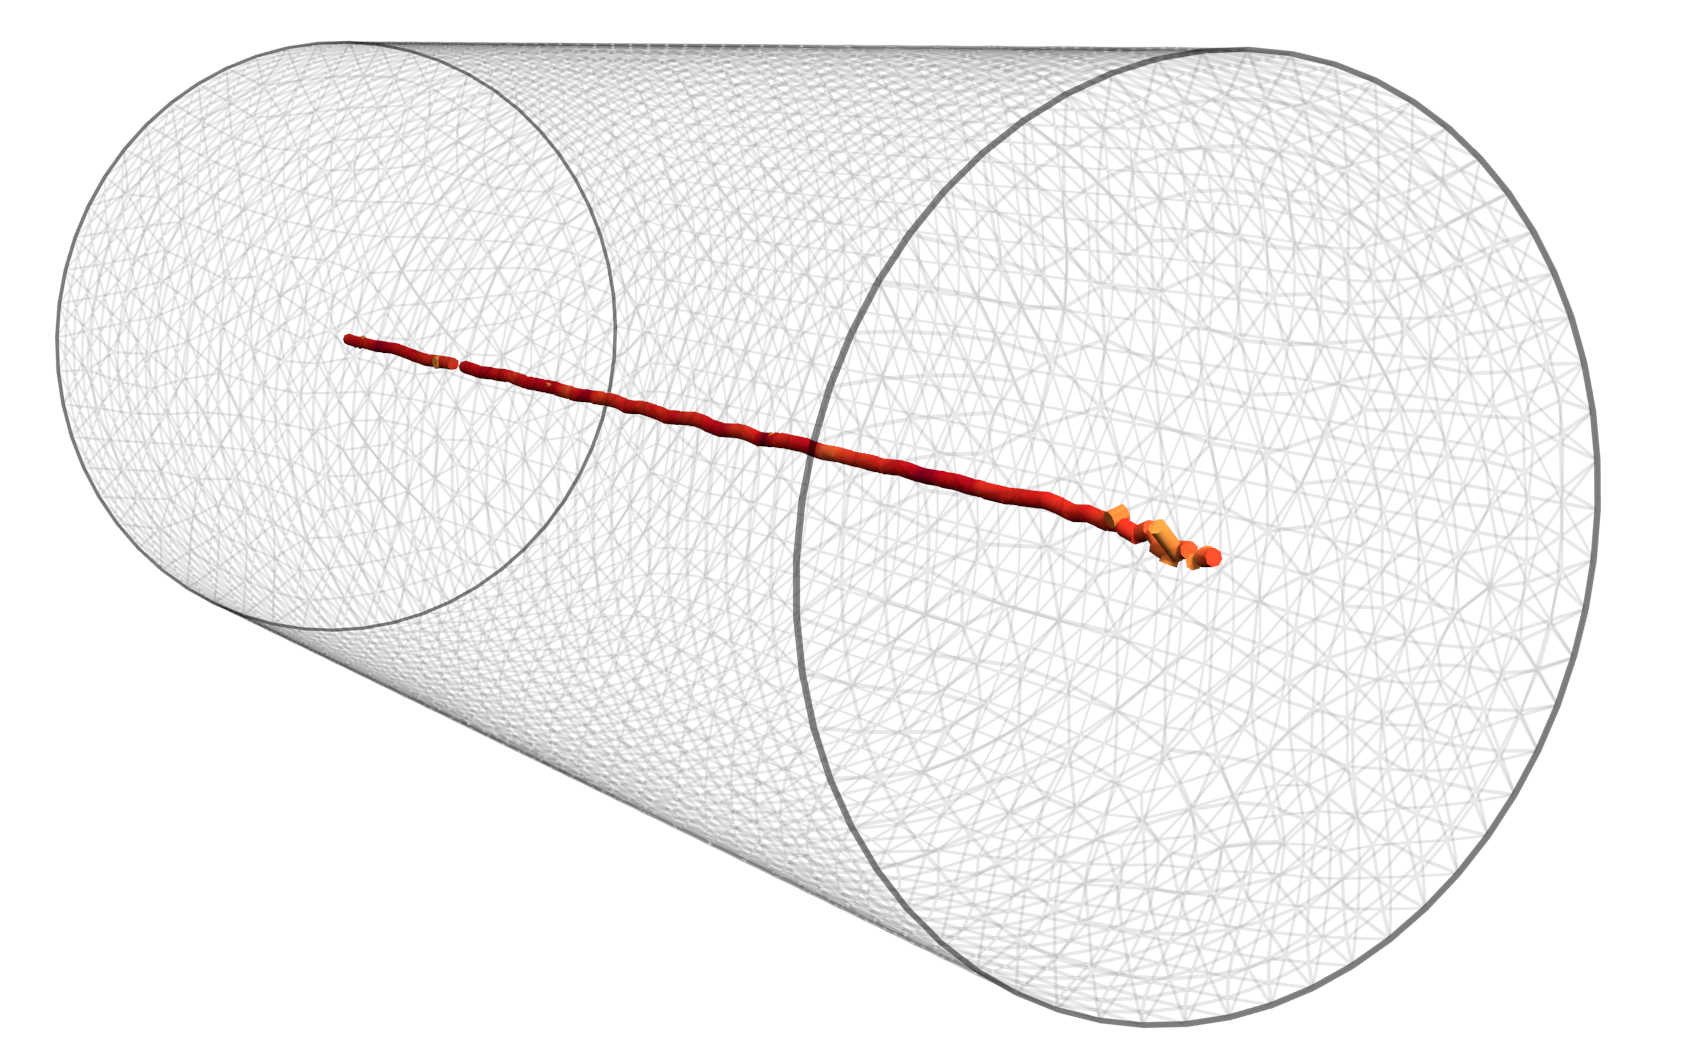
\includegraphics[width=0.45\figurewidth]{figures/cylinder_lines_m100}%
    };
    \node[anchor=south west] at (image1.south west) {\small $M = \num{100}$};

    \node[image, right=of image1] (image2)
    {
        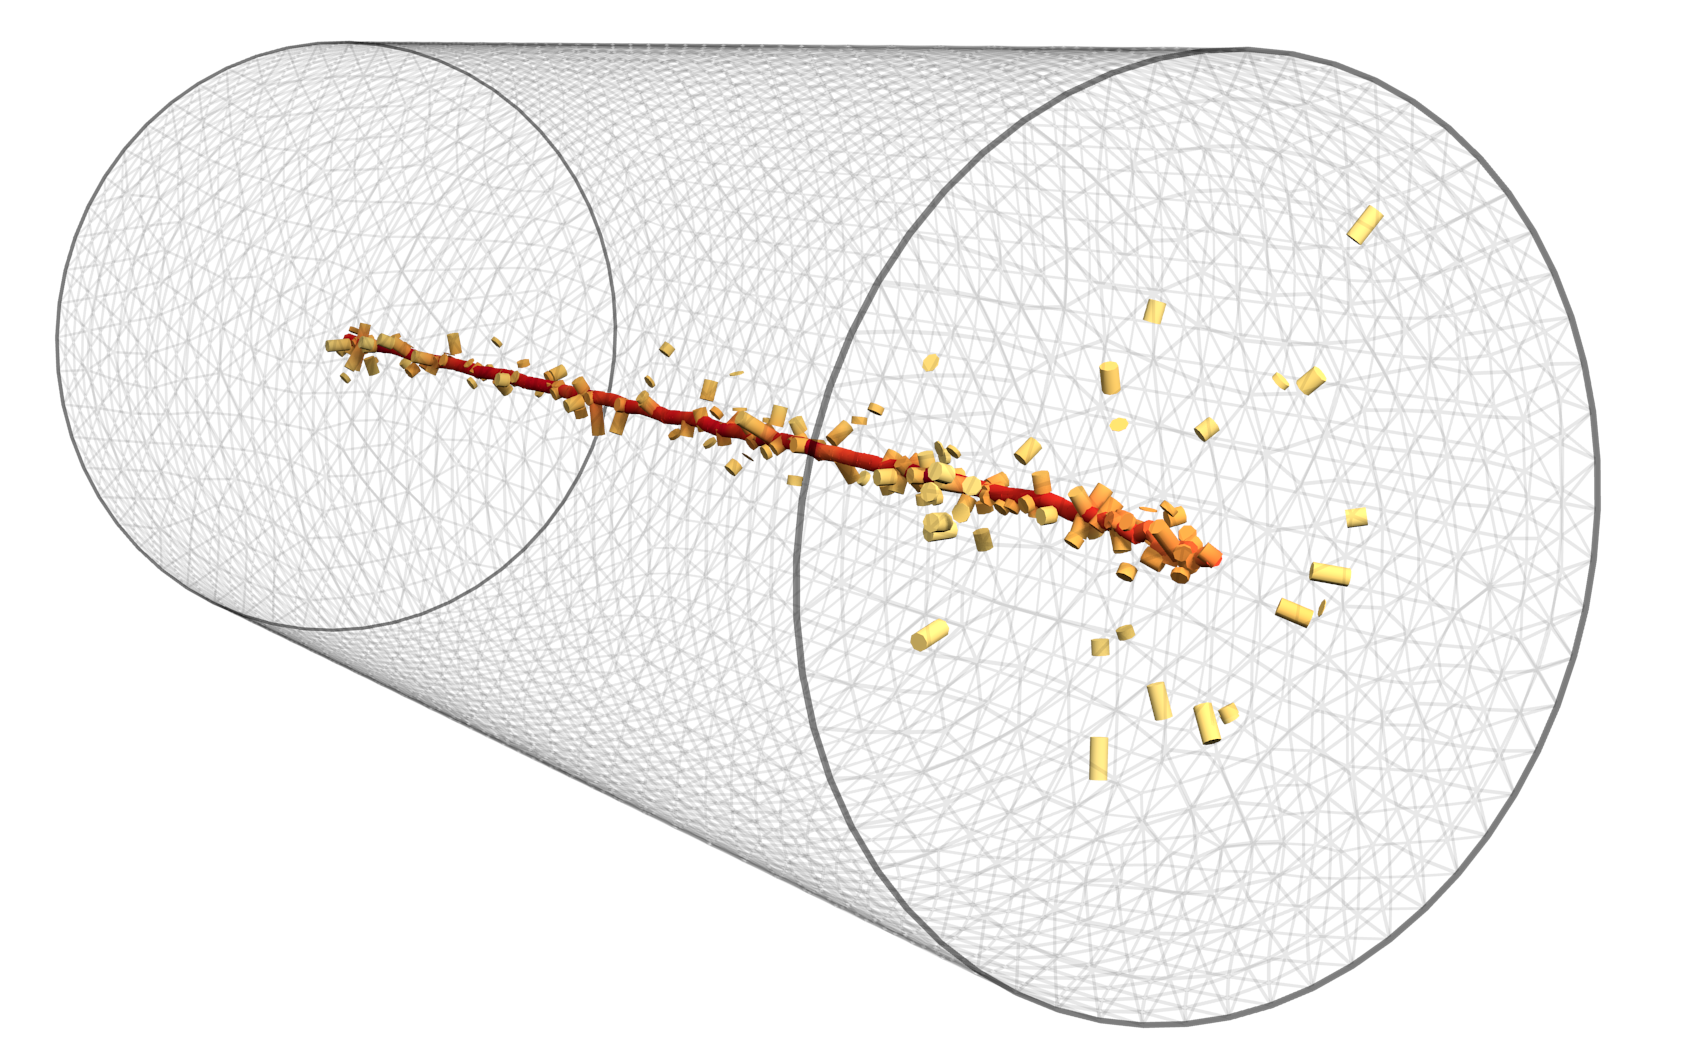
\includegraphics[width=0.45\figurewidth]{figures/cylinder_lines_m1000}%
    };
    \node[anchor=south west] at (image2.south west) {\small $M = \num{1000}$};

    \node[image, below=of image1, yshift=-0.1cm] (image3)
    {
        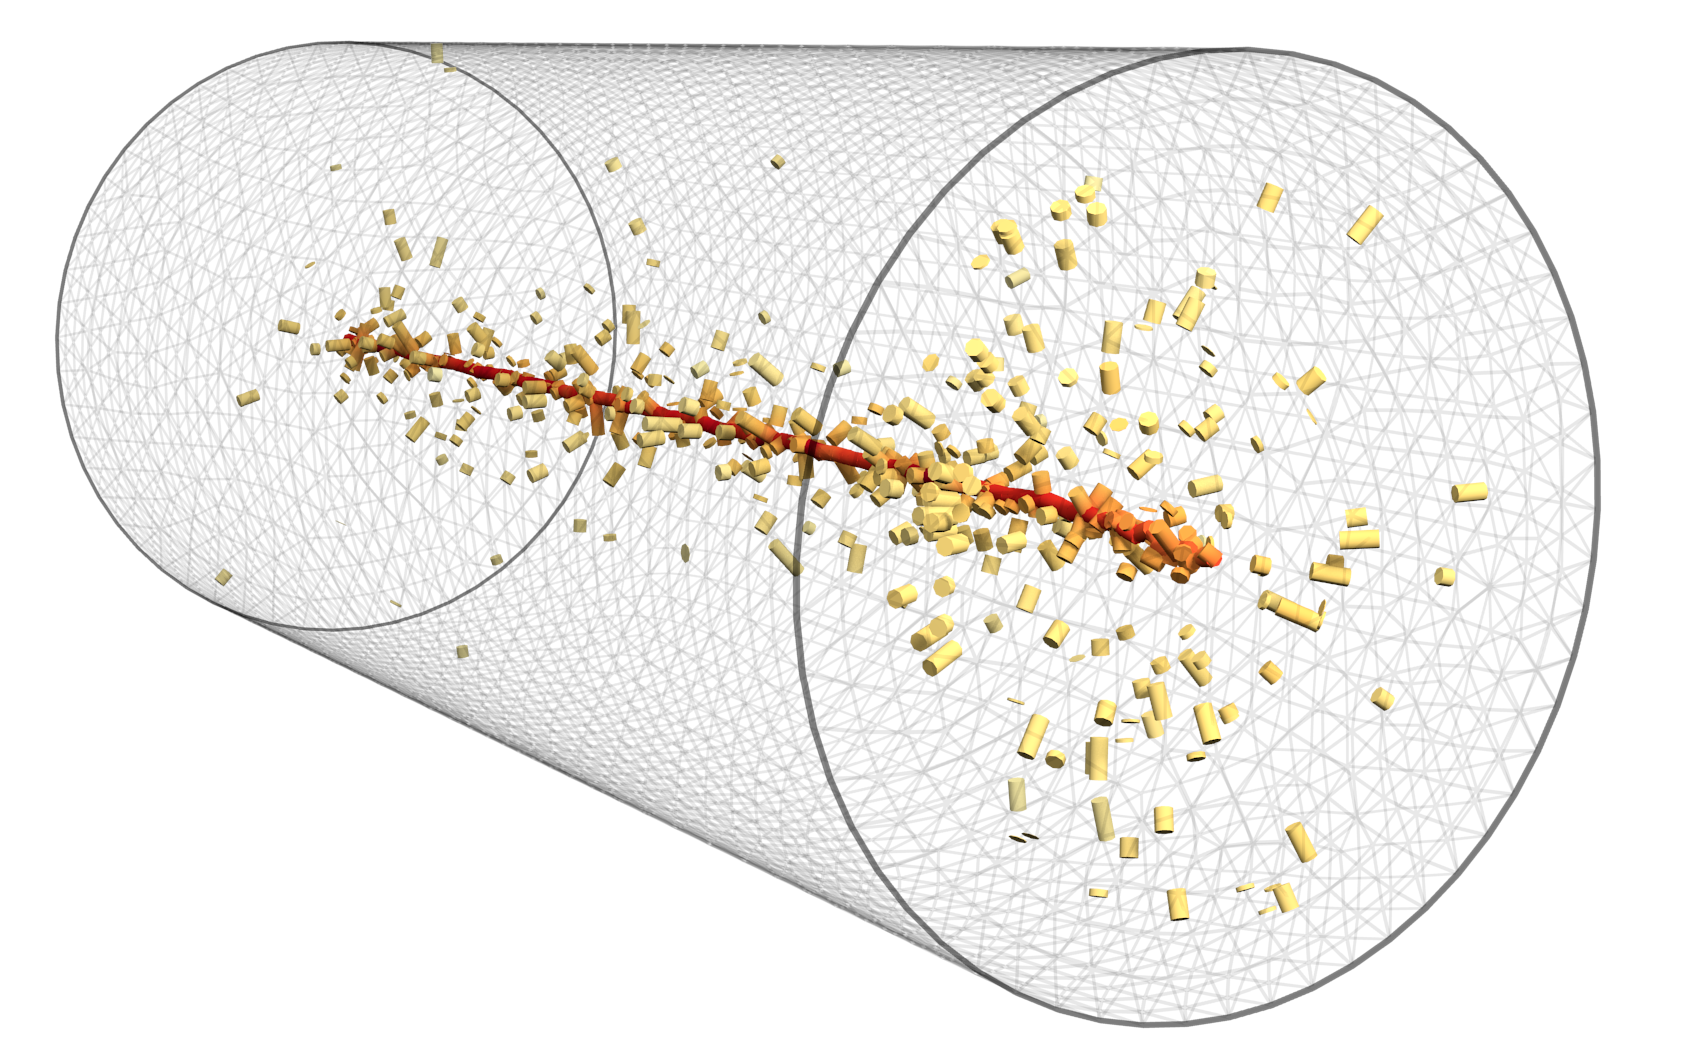
\includegraphics[width=0.45\figurewidth]{figures/cylinder_lines_m10000}%
    };
    \node[anchor=south west] at (image3.south west) {\small $M = \num{10000}$};

    \node[image, right=of image3] (image4)
    {
        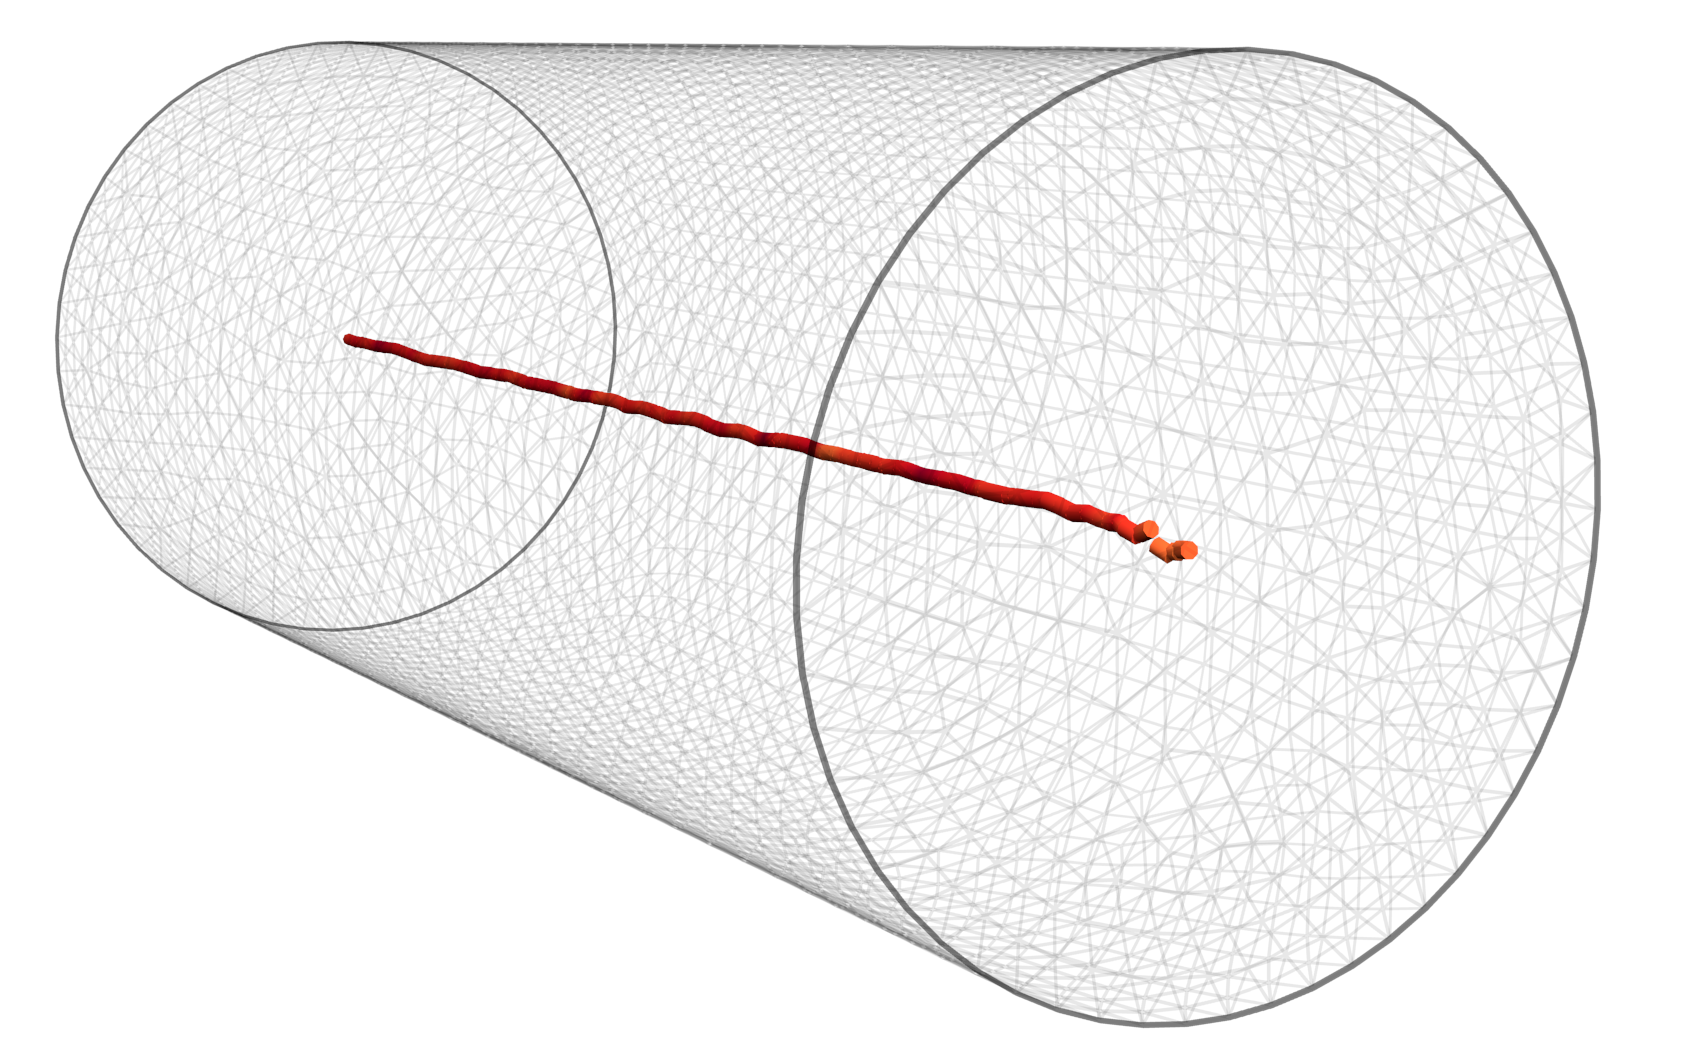
\includegraphics[width=0.45\figurewidth]{figures/cylinder_lines_filtered}%
    };
    \node[anchor=south west] at (image4.south west) {\small filtered};

    \node[anchor=west, xshift=-0.75cm] at (image4.north east){
        \begin{axis}[
        scale only axis,
        height=4cm,
        hide axis,
        domain=1:20,
        colorbar,
        colorbar/width=0.25cm,
        colormap name={rdoryl},
        point meta min=1, point meta max=20,
        colorbar style={
            title=$\log(s)$,
            scaled ticks=false,
            ytick={1, 20}
        }]
      \end{axis}
    };

\end{tikzpicture}
    \vspace*{-5mm}
    \caption{Results of our algorithm on the \textsc{Cylinder} dataset for
             different choices of $M$. Increasing $M$ results in more
             numerically unstable lines being found. If we filter them out, the
             result is virtually identical.}
    \label{fig:unfiltered_lines}
\end{figure}
%
% subsection performance (end)
%
\subsection{Comparison with Degenerate Lines} % (fold)
\label{sub:comparison_with_degenerate_lines}
%
Tensor core lines are mathematically distinct from degenerate lines where two or
more eigenvalues are equal.
%
The criterion for finding tensor core lines is completely independent of the
eigenvalues of the tensor field.
%
However, when looking at our results in stress tensor fields, one might wonder
if tensor core lines coincide with degenerate lines in practice.
%
To investigate this, we extracted degenerate lines from our datasets using the
method presented by Zheng and Pang \cite{Zheng2004}.
%
In stress tensor fields, degenerate lines mark locations where no unique
principal directions of stress can be established.
%
We found that tensor core lines and degenerate lines sometimes coincide, but
neither is a subset of the other.
%
In the \textsc{Crane} dataset, degenerate lines are found near the center of the
lower diagonal rods, where we also find tensor core lines.
%
However, a lot of degenerate lines are also found in regions where no tensor
core lines are located.
%
In the \textsc{Truck Bumper} dataset, a degenerate line coincides with one of
the two most significant tensor core lines we find, but not the other one.
%
Closeups of both datasets are shown in~\cref{fig:topo_comparison}.
%
In several datasets, such as the \textsc{Cylinder} and \textsc{Handle}, Zheng
and Pang's method fails to locate any degenerate lines at all.
%
\begin{figure}[p]
    \begin{captionbeside}{Comparison of unfiltered tensor core lines
    (red/yellow) and degenerate tensor lines (blue) for the \textsc{Truck
    Bumper} and \textsc{Crane} dataset. The red box marks the
    coincidence of a numerically stable tensor core line with a degenerate
    tensor line.\label{fig:topo_comparison}}
        \setlength{\figurewidth}{0.7\textwidth}
        %
\begin{tikzpicture}[
    image/.style={inner sep=0, outer sep=0, node distance = 0 and 0},
    label/.style={anchor=north west, fill=white, font=\small, xshift=1mm, yshift=-1mm}
]

    \node[image, anchor=south west] (image1)
    {
        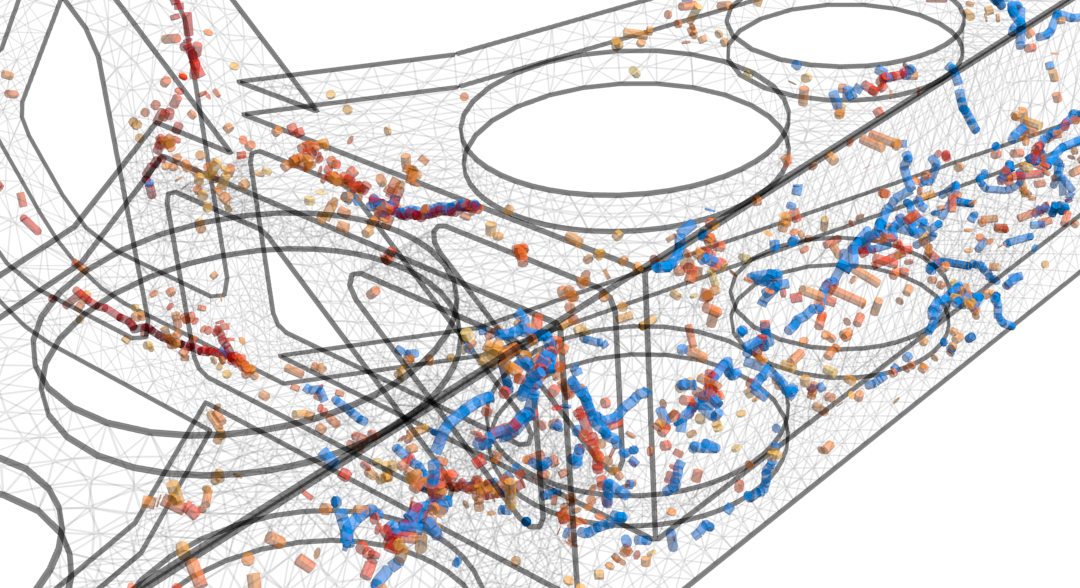
\includegraphics[width=\figurewidth]{figures/truck_bumper_topo_lines_detail2_slim}%
    };
    \begin{scope}[
        shift=(image1.south west), % origin is lower left corner
        x={($(image1.south east)-(image1.south west)$)}, % x axis is lower side
        y={($(image1.north west)-(image1.south west)$)}] % y axis is left side
        % \draw[help lines,xstep=.1,ystep=.1] (0,0) grid (1,1);
        % \foreach \x in {0,1,...,9} { \node [anchor=north] at (\x/10,0) {\scriptsize 0.\x}; }
        % \foreach \y in {0,1,...,9} { \node [anchor=east] at (0,\y/10) {\scriptsize 0.\y}; }
        \draw[red,very thick,rounded corners] (0.3,0.57) rectangle (0.47,0.68);
    \end{scope}
    \node[label] at (image1.north west) {\textsc{Truck Bumper}};

    \node[image, below=of image1, yshift=-0.2cm] (image2)
    {
        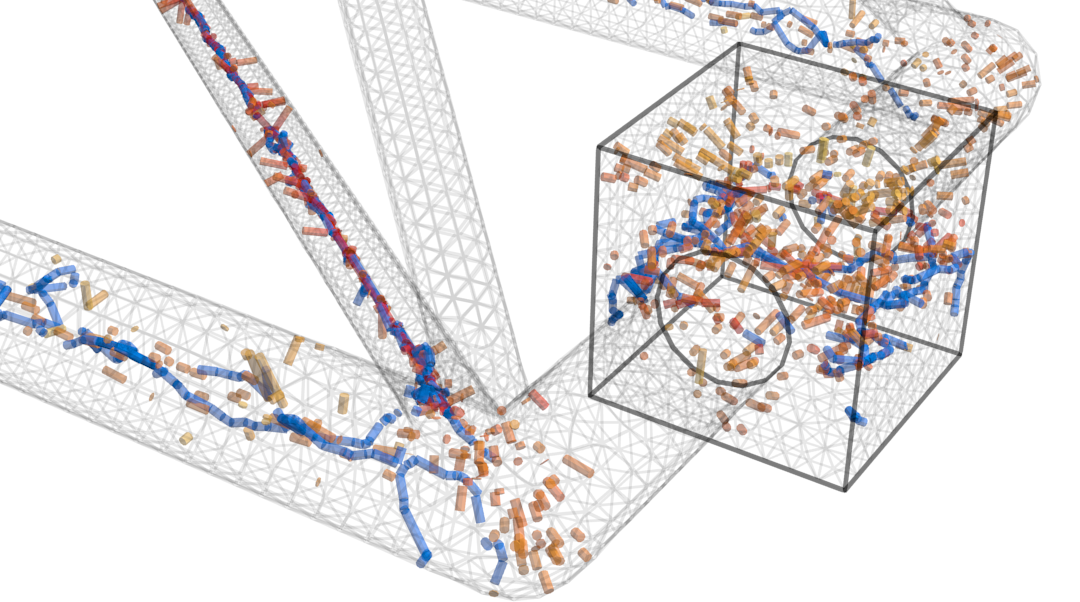
\includegraphics[width=\figurewidth]{figures/crane_topo_lines_detail1_slim}%
    };
    \begin{scope}[
        shift=(image2.south west), % origin is lower left corner
        x={($(image2.south east)-(image2.south west)$)}, % x axis is lower side
        y={($(image2.north west)-(image2.south west)$)}] % y axis is left side
        % \draw[help lines,xstep=.1,ystep=.1] (0,0) grid (1,1);
        % \foreach \x in {0,1,...,9} { \node [anchor=north] at (\x/10,0) {\scriptsize 0.\x}; }
        % \foreach \y in {0,1,...,9} { \node [anchor=east] at (0,\y/10) {\scriptsize 0.\y}; }
        \draw[mycolor4, very thick, rotate around={-57:(0.295, 0.66)}]
            (0.295, 0.66) ellipse (0.21 and 0.04);
    \end{scope}
    \node[label] at (image2.north west) {\textsc{Crane}};
\end{tikzpicture}
    \end{captionbeside}
\end{figure}
%
% subsection comparison_with_degenerate_lines (end)
%
% section results (end)
%
\section[Computing PEV and Degenerate Lines]%
{Computing \ac{PEV} and Degenerate Lines} % (fold)
\label{sec:computing_pev_and_degenerate_lines}
%
The algorithm we have presented for extracting tensor core lines is a generic
root finding algorithm adapted to find simultaneous roots of multiple
polynomials.
%
Because of its genericity, we can also use it to extract \ac{PEV} lines and
degenerate lines, which can be expressed as root finding problems of the same
type.
%
This makes it possible to extract several different feature lines from tensor
fields using the same algorithmic framework.
%

%
We remember the criterion for \ac{PEV} lines of two tensor fields $\mS$ and
$\mT$. A \ac{PEV} line passes through every point $\vx$ that satisfies
%
\begin{equation*}
    \vr \parallel \mS(\vx)\,\vr \parallel \mT(\vx)\,\vr \,\text{.}
\end{equation*}
%
Again using the fact that the cross product of two parallel vectors is zero, we
translate this to the system of polynomials
%
\begin{equation}
    \begin{aligned}
        (\mS(\vx)\,\vr) \times \vr &= \vNull\\
        (\mT(\vx)\,\vr) \times \vr &= \vNull \,\text{.}\\
    \end{aligned}
\end{equation}
%
This system has six polynomials that are quadratic in $\vr$ and linear in $\vx$,
which need to become zero at the same time.
%
We can use the same recursive subdivision algorithm based on the
Bernstein-B\'ezier forms of these polynomials to find solutions.
%

%
Computing \ac{PEV} lines using this scheme has several advantages.
%
The algorithm is somewhat simpler than the one we presented in
\cref{sec:extracting_pev_lines}, as no two separate nested recursive processes
are required.
%
This means that is is simpler to explain and implement.
%
More importantly, using this algorithm does not result in false-positive
solution candidates that need to be filtered out.
%
Computing times using this algorithm are however somewhat longer.
%
This is because the separate recursion in $\vr$-space that is used in the
original \ac{PEV} algorithm can frequently be terminated early while the
subdivision level in $\vx$-space is still low.
%
This is not possible in the root finding algorithm we presented here, as it
considers both spaces simultaneously.
%

%
The extraction of degenerate lines in tensor fields can be expressed as a root
finding problem as well.
%
A degenerate line is located where two eigenvalues of a tensor field are equal.
%
Zheng \etal{}~\cite{Zheng2004} showed that these locations can be expressed as the
simultaneous roots of the seven \emph{discriminant constraint functions}
%
\begin{equation}
    \begin{aligned}
        f_x(\mT) &= T_{00}(T^2_{11} - T^2_{22}) + T_{00}(T^2_{01} - T^2_{02}) +
                    T_{11}(T^2_{22} - T^2_{00}) + T_{11}(T^2_{12} - T^2_{01})\\
                    &\phantom{{}={}}  + T_{22}(T^2_{00} - T^2_{11})
                    + T_{22}(T^2_{02} - T^2_{12})\\
        f_{y1}(\mT) &= T_{12}\left(2(T^2_{12} - T^2_{00}) - (T^2_{02} + T^2_{01}) +
                    2(T_{11}T_{00} + T_{22}T_{00} - T_{11}T_{22})\right)\\
                    &\phantom{{}={}}+ T_{01}T_{02}(2 T_{00} - T_{22} - T_{11})\\
        f_{y2}(\mT) &= T_{02}\left(2(T^2_{02} - T^2_{11}) - (T^2_{01} + T^2_{12})
                    + 2(T_{22}T_{11} + T_{00}T_{11} -T_{22}T_{00})\right) \\
                    &\phantom{{}={}}+ T_{12}T_{01}(2T_{11} - T_{00} - T_{22})\\
        f_{y3}(\mT) &= T_{01}\left(2(T^2_{01} - T^2_{22}) - (T^2_{12} + T^2_{02})
                    + 2(T_{00}T_{22} + T_{11}T_{22} -T_{00}T_{11})\right) \\
                    &\phantom{{}={}}+ T_{02}T_{12}(2T_{22} - T_{11} - T_{00})\\
        f_{z1}(\mT) &= T_{12}(T^2_{02} - T^2_{01}) + T_{01}T_{02}(T_{11} - T_{22})\\
        f_{z2}(\mT) &= T_{02}(T^2_{01} - T^2_{12}) + T_{12}T_{01}(T_{22} - T_{00})\\
        f_{z3}(\mT) &= T_{01}(T^2_{12} - T^2_{02}) + T_{02}T_{12}(T_{00} - T_{11})\,\text{,}
    \end{aligned}
\end{equation}
%
where $\mT = \mT(\vx)$ is the tensor field and $T_{ij}$ are the components of
the (symmetric) tensor.
%
The advantage of using these functions is that it does not require the explicit
computation of eigenvalues.
%
We can find the simultaneous roots of these seven polynomials that are maximum
cubic in $\vx$ using the same scheme we used to extract tensor core lines.
%
Since these equations do not depend on a direction $\vr$, we only need to
subdivide in $\vx$-space.
%
The degenerate lines shown in \cref{fig:topo_comparison} were computed in this
way.
%

%

%
% section computing_pev_and_degenerate_lines (end)
%
%
\section{Discussion} % (fold)
\label{sec:tcl_discussion}
%
We introduced tensor core lines as a new feature of second-order tensor fields.
%
It enables the quick detection of swirling behavior in tensor field lines.
%
Such behavior might not have a distinct physical meaning in all applications.
%
However, finding core lines helps to understand the structure of the tensor
field by breaking down a complex feature into a simple line structure that can
be easily visualized.
%
In this regard, our method fits in well with other feature-based visualization
methods.
%

%
Our method is a direct extension of the Sujudi/Haimes method for the extraction
of vortex core lines in vector fields.
%
As such, it shares many of its advantages and drawbacks.
%
The criterion is completely local and does not require integration.
%
As such, it is well parallelizable and not vulnerable to accumulating numerical
errors.
%
Still, we are hardly able to reach interactive run times, as we need to perform
an exhaustive search in a \ac{5D} space.
%
Like Sujudi/Haimes, we perform a search on piecewise linear data, which results
in straight lines within cells and discontinuities of the tensor core lines at
cell boundaries.
%
Using higher-order interpolation of the tensor field would help finding
continuous lines.
%

%
We have chosen to focus on piecewise linear tensor fields where each tensor
component is interpolated independently.
%
While alternative interpolation schemes have been proposed~\cite{Kindlmann2007},
component-wise interpolation is still widely used as a standard approach for
both tensor- and vector fields.
%

%
Unlike Sujudi/Haimes, we have no way of explicitly ensuring our solutions show
only swirling behavior by restricting them to regions where the derivative has
complex eigenvalues.
%
The derivative of the tensor field $\nabla \mT$ is a third-order tensor, for
which the definition of eigenvalues and eigenvectors is non-trivial
\cite{Zheng2007}.
%
This means that we also find structures similar to hyperbolic trajectories in
vector fields \cite{Machado2013,Machado2016}.
%
Further research is necessary in order to distinguish these different types of
features.
%

%
We introduced a measure for the numeric stability of tensor core lines.
%
Unfortunately, filtering out numerically unstable solutions must be done as an
interactive post-processing step, as the threshold is different for each
dataset.
%
It is worth investigating if this process can be automated.
%
Nevertheless, the measure enables us to distinguish significant and
insignificant solutions, which is a very useful tool for assessing the result of
our algorithm.
%

%
Our algorithm is numerically very stable.
%
We have three free parameters, two of which can be chosen in a wide range
without significant influence on the results, as we show in
\cref{sub:performance}.
%
The parameter $M$, which influences run time the most, can be chosen the same
for most datasets and as such does not require fine-tuning either.
%

%
Our algorithm is only designed for extracting structurally stable line
features, but surfaces or regions where the zero curvature criterion is
almost fulfilled seem to be common in real-world stress tensor data.
%
This might be due to the common occurrence of symmetries and regular shapes in
human-made objects, which are most frequently the focus of structural analysis.
%
It would therefore be interesting to investigate if these structures can
explicitly be extracted, possibly by restricting the search space to the edges
of tetrahedral cells.
%

%
Finally, it is worth noting that neither the formal definition of tensor core
lines nor the extraction algorithm poses any restrictions on the tensor field,
except that it be differentiable.
%
As such, it might also be used on indefinite tensor data, such as the Jacobian
of a vector field.
%
Finding applications outside of stress tensor analysis is a subject for further
research.
%
%
% chapter tensor_core_lines (end)